\documentclass{beamer}
\usetheme{Boadilla}  %% Themenwahl

\title{Erweiterung eines Frameworks zur Generierung freier Theoreme um Typkonstruktorklassen}
\author{Thomas Rossow}
\date{22. Februar 2017}

\usepackage[utf8]{inputenc} % set input encoding (not needed with XeLaTeX)
\usepackage{minted}

\AtBeginSection[]{
  \begin{frame}
  \vfill
  \centering
  \begin{beamercolorbox}[sep=8pt,center,shadow=true,rounded=true]{title}
    \usebeamerfont{title}\insertsectionhead\par%
  \end{beamercolorbox}
  \vfill
  \end{frame}
}

\beamertemplatenavigationsymbolsempty
\setbeamertemplate{footline}{\hfill\makebox[24pt]{\scriptsize\insertframenumber/\inserttotalframenumber}}

\begin{document}
\maketitle
\frame{\tableofcontents}

% % % % % % % % % % % % % % % % % % % % % % % % % % % % % % %
\section{Was ist ein freies Theorem?}
% % % % % % % % % % % % % % % % % % % % % % % % % % % % % % %

\begin{frame}
\frametitle{Was ist ein freies Theorem?}
%\texttt{f :: [a] $\rightarrow$ [a]}

\begin{itemize}
\item Aussage zu beliebiger Typsignatur
\item Zu jeder Typsignatur lässt sich freies Theorem herleiten
\end{itemize}
\end{frame}

% - - - - - - - - - - - - - - - - - - - - - - - - - - - - - - - - - - - - - - - - - - - - - - - - - - - - - - - - - - - - 

\begin{frame}[fragile]
\frametitle{Freie Theoreme: Beispiel}
\begin{minted}{haskell}
f :: forall a. [a] -> [a]
\end{minted}

\pause

Für alle Funktionen $g : T_1 \rightarrow T_2$ und Listen $l :: [T_1]$ gilt:

\begin{align*}
f\ (map\ g\ l) = map\ g\ (f\ l)
\end{align*}
\end{frame}

% - - - - - - - - - - - - - - - - - - - - - - - - - - - - - - - - - - - - - - - - - - - - - - - - - - - - - - - - - - - - 

\begin{frame}
\frametitle{Freie Theoreme: Beispiel}

\begin{center}
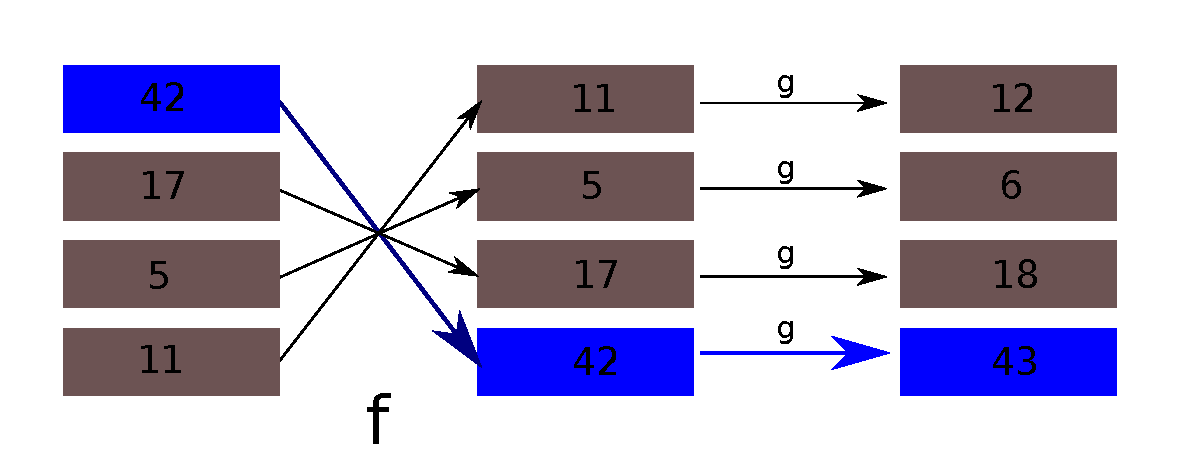
\includegraphics[width=300px]{fmapg}
\end{center}

\end{frame}

% - - - - - - - - - - - - - - - - - - - - - - - - - - - - - - - - - - - - - - - - - - - - - - - - - - - - - - - - - - - - 

\begin{frame}
\frametitle{Freie Theoreme: Beispiel}

\begin{center}
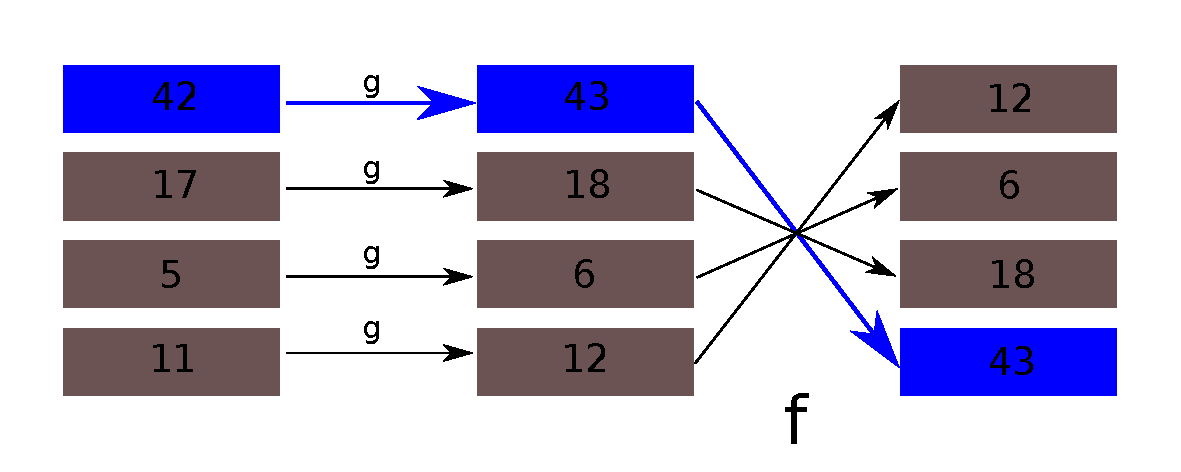
\includegraphics[width=300px]{mapgf}
\end{center}

\end{frame}


% % % % % % % % % % % % % % % % % % % % % % % % % % % % % % %
\section{Die Theorie hinter freien Theoremen}
% % % % % % % % % % % % % % % % % % % % % % % % % % % % % % %

\begin{frame}
\frametitle{Die Theorie hinter freien Theoremen}

\begin{itemize}
\item Auffassen von Typen als Relationen
\item Parametrizitätstheorem
\end{itemize}
\end{frame}

% - - - - - - - - - - - - - - - - - - - - - - - - - - - - - - - - - - - - - - - - - - - - - - - - - - - - - - - - - - - - 

\begin{frame}[fragile]
\frametitle{Beispielstruktur}
\begin{minted}{haskell}
data OnetoFive = One | Two | Three | Four | Five

plusOne :: OnetoFive -> OnetoFive
plusOne One = Two
plusOne Two = Three
...

doubleIt :: OnetoFive -> OnetoFive
doubleIt One = Two
doubleIt Two = Four
...

plusTwo :: OnetoFive -> OnetoFive
halfOf :: OnetoFive -> OnetoFive
\end{minted}
\end{frame}

% - - - - - - - - - - - - - - - - - - - - - - - - - - - - - - - - - - - - - - - - - - - - - - - - - - - - - - - - - - - - 

\begin{frame}
\frametitle{Repräsentation von Typen}

\begin{itemize}
\item Möglichkeit: Typen als Mengen auffassen
\item Beispiel: \texttt{Int} aufgefasst als $\mathbb{N}$
\end{itemize}

\begin{center}
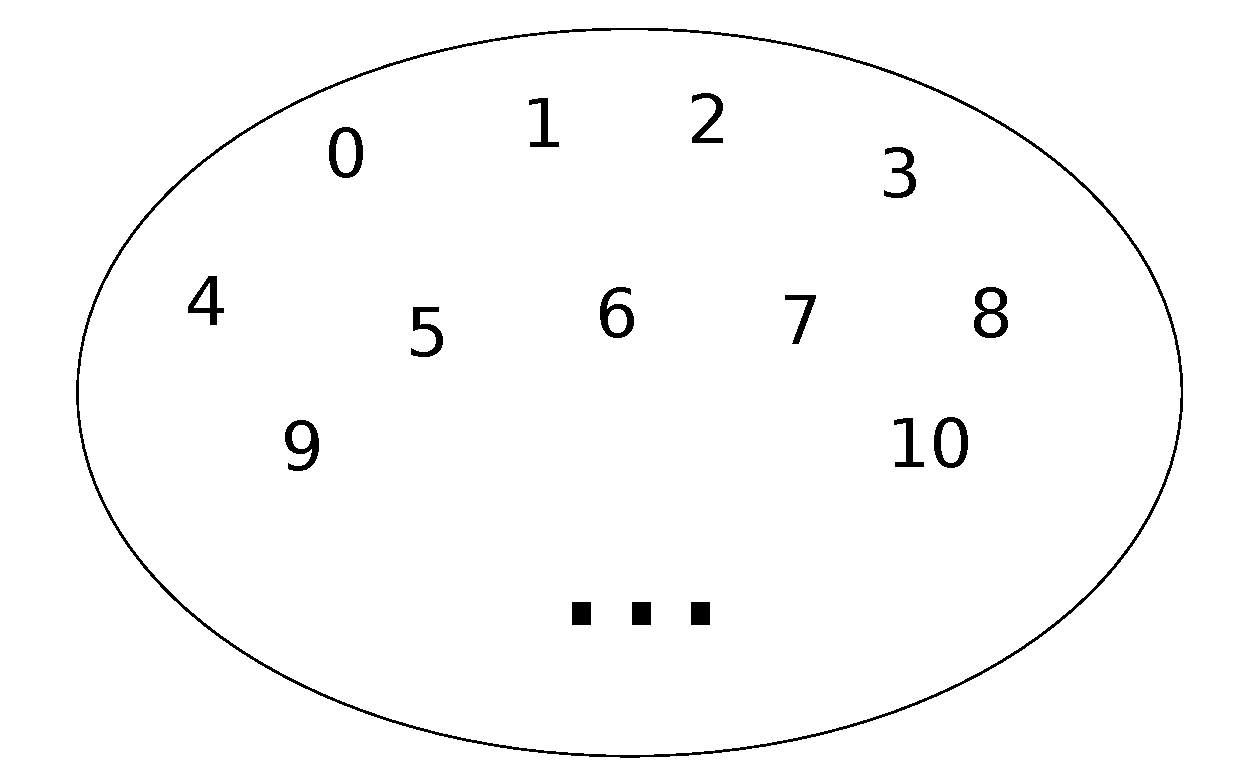
\includegraphics[width=250px]{menge-n}
\end{center}
\end{frame}

% - - - - - - - - - - - - - - - - - - - - - - - - - - - - - - - - - - - - - - - - - - - - - - - - - - - - - - - - - - - - 

\begin{frame}
\frametitle{Repräsentation von Typen}

\begin{center}
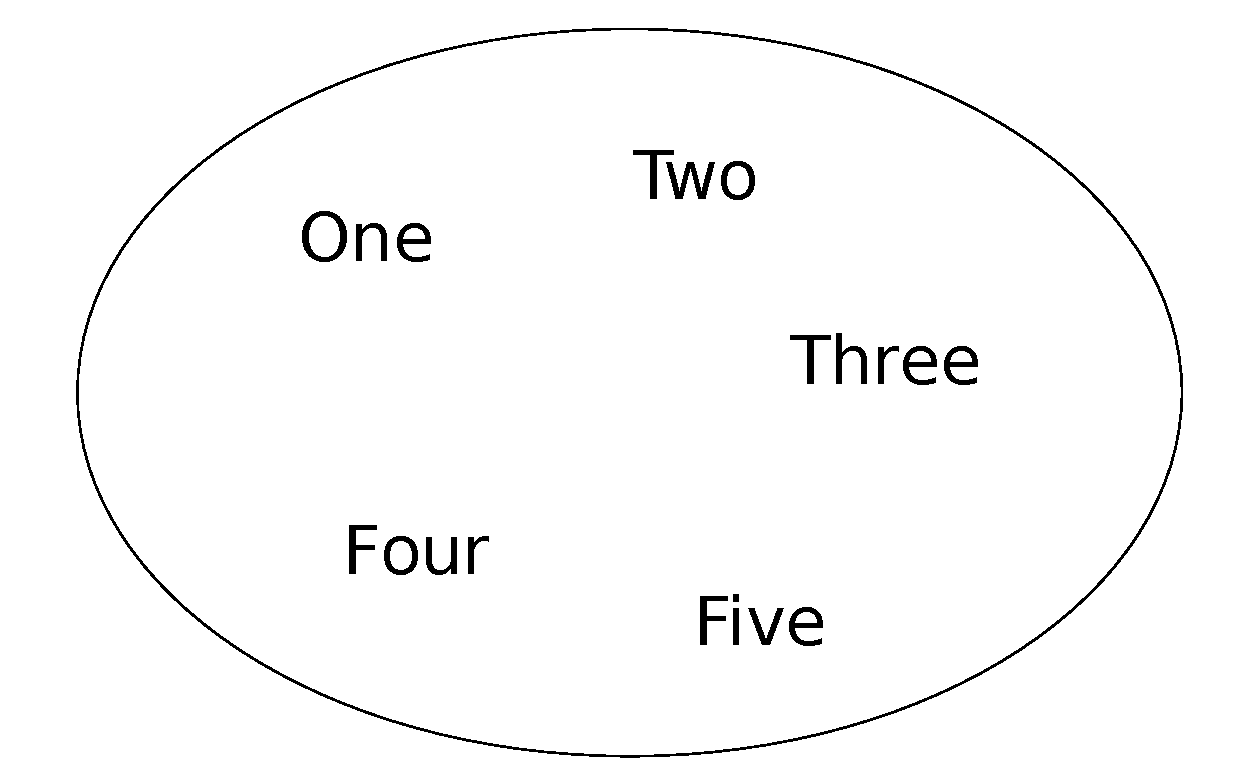
\includegraphics[width=250px]{menge-onetofive}
\end{center}
\end{frame}

% - - - - - - - - - - - - - - - - - - - - - - - - - - - - - - - - - - - - - - - - - - - - - - - - - - - - - - - - - - - - 

\begin{frame}
\frametitle{Repräsentation von Typen}

\begin{itemize}
\item Andere Möglichkeit: als Relationen auf Typmengen
\item Verwandtheit von Ausdrücken $\Leftrightarrow$ Überführbarkeit
\end{itemize}
\end{frame}

% - - - - - - - - - - - - - - - - - - - - - - - - - - - - - - - - - - - - - - - - - - - - - - - - - - - - - - - - - - - - 

\begin{frame}[fragile]
\frametitle{Typen als Relationen}

\begin{itemize}
\item Zu jeder Typsignatur lässt sich Relation konstruieren
\end{itemize}

\pause
\vspace{36px}
Beispiel

\begin{minted}{haskell}
f :: forall a b. (a -> b) -> a -> b
\end{minted}

\pause

$\forall ~\mathcal{R} ~\mathcal{S}.~ (\mathcal{R} \rightarrow \mathcal{S}) \rightarrow \mathcal{R} \rightarrow \mathcal{S}$
\end{frame}

% - - - - - - - - - - - - - - - - - - - - - - - - - - - - - - - - - - - - - - - - - - - - - - - - - - - - - - - - - - - - 

\begin{frame}
\frametitle{Relationale Aktionen}

\begin{itemize}
\item Man definiert ``relationale Aktionen''
\item Ordnen Typkonstruktor und Relationen neue Relation zu
\end{itemize}

\pause
\vspace{36px}
Beispiele

\begin{itemize}[<+->]
\item $\mathcal{R} \rightarrow \mathcal{S}$ (Funktionskonstruktor)
\item $\forall \mathcal{R}.~ A(\mathcal{R})$ (Typabstraktion)
\item $[\mathcal{R}]$ (Listentypkonstruktor)
\end{itemize}

\end{frame}


% - - - - - - - - - - - - - - - - - - - - - - - - - - - - - - - - - - - - - - - - - - - - - - - - - - - - - - - - - - - - 

\begin{frame}[fragile]
\frametitle{Relationale Aktionen: Basistypen}

Relation zu Basistypen ist die Identitätsrelation

\pause
\vspace{36px}
Beispiel:

\begin{minted}{haskell}
n :: OnetoFive
\end{minted}

\pause

$\Rightarrow~id_{OnetoFive}$

\end{frame}

% - - - - - - - - - - - - - - - - - - - - - - - - - - - - - - - - - - - - - - - - - - - - - - - - - - - - - - - - - - - - 

\begin{frame}
\frametitle{Relationale Aktionen: Basistypen}

\begin{center}
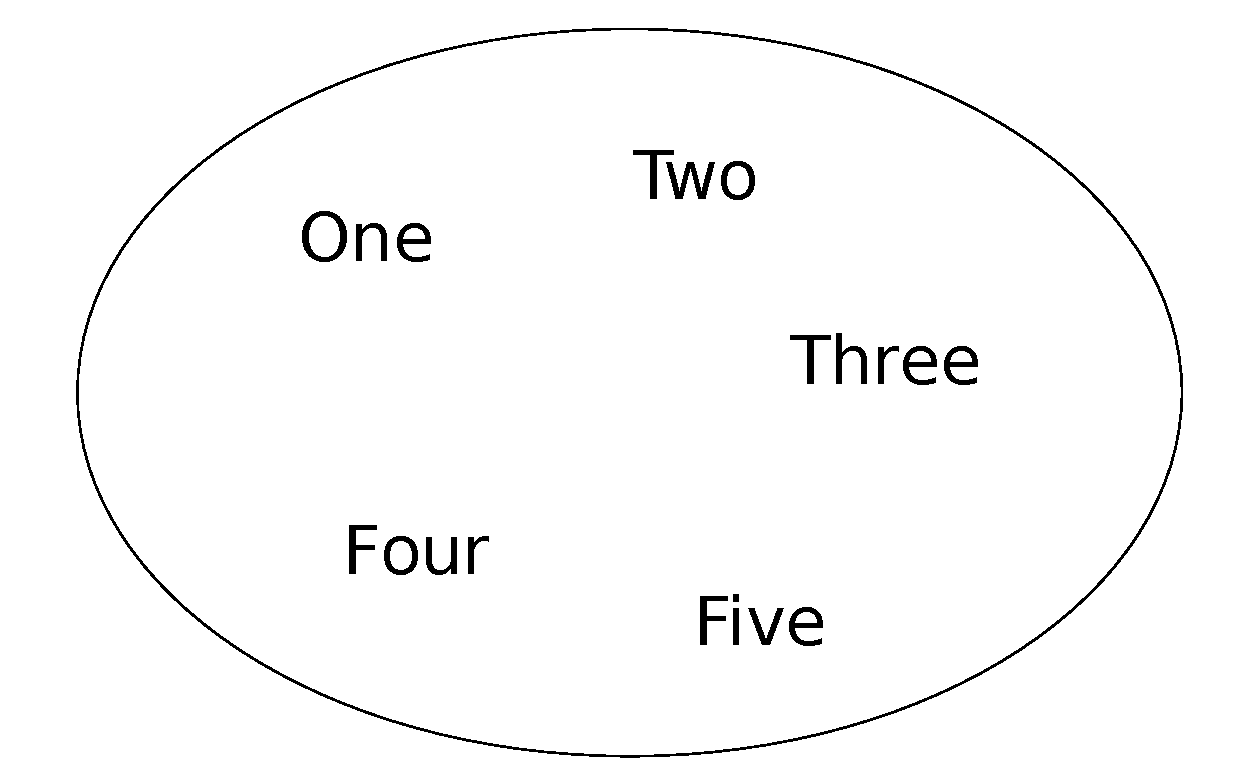
\includegraphics[width=250px]{menge-onetofive}
\end{center}

\vspace{63.5px}

\end{frame}

% - - - - - - - - - - - - - - - - - - - - - - - - - - - - - - - - - - - - - - - - - - - - - - - - - - - - - - - - - - - - 

\begin{frame}
\frametitle{Relationale Aktionen: Basistypen}

\begin{center}
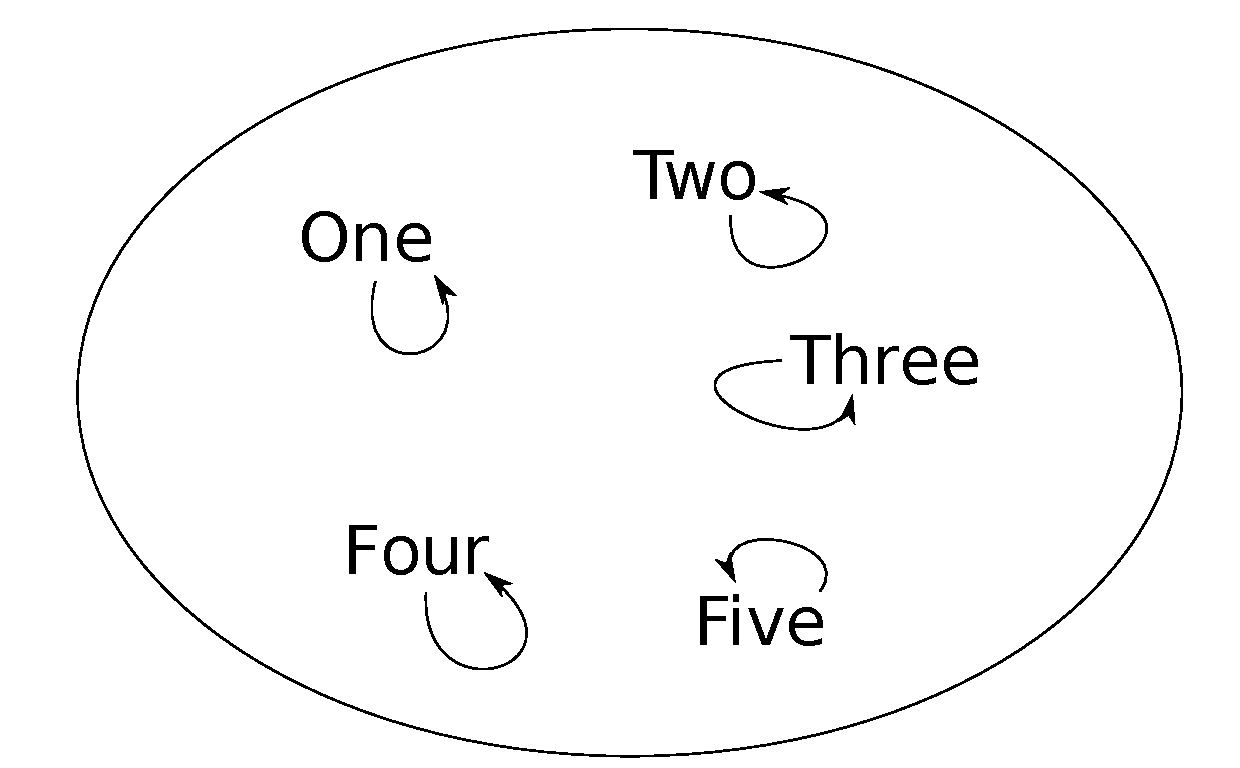
\includegraphics[width=250px]{relation-onetofive}
\end{center}

\pause

\begin{align*}
id_{OnetoFive} = \{ (One, One), (Two, Two), (Three, Three),\\
(Four, Four), (Five, Five) \}
\end{align*}

\end{frame}

% - - - - - - - - - - - - - - - - - - - - - - - - - - - - - - - - - - - - - - - - - - - - - - - - - - - - - - - - - - - - 

\begin{frame}[fragile]
\frametitle{Relationale Aktionen: Funktionen}

Funktionen, die verwandte Werte auf verwandte Werte abbilden, sind verwandt.

\vspace{36px}

Beispiel:

\begin{minted}{haskell}
f :: OnetoFive -> OnetoFive
\end{minted}

\pause

$id_{OnetoFive} \rightarrow id_{OnetoFive}$

\end{frame}

% - - - - - - - - - - - - - - - - - - - - - - - - - - - - - - - - - - - - - - - - - - - - - - - - - - - - - - - - - - - - 

\begin{frame}
\frametitle{Relationale Aktionen: Funktionen}

\begin{center}
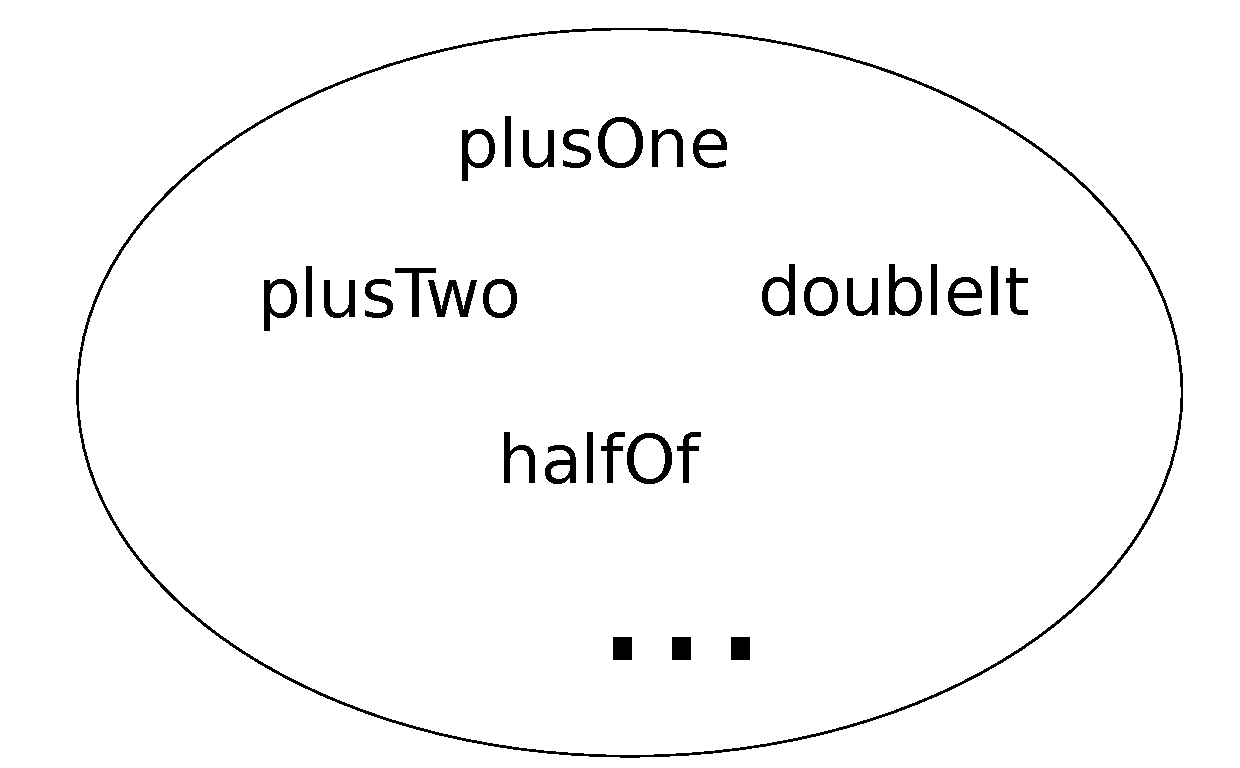
\includegraphics[width=250px]{menge-onetofive-functions}
\end{center}
\end{frame}

% - - - - - - - - - - - - - - - - - - - - - - - - - - - - - - - - - - - - - - - - - - - - - - - - - - - - - - - - - - - - 

\begin{frame}
\frametitle{Relationale Aktionen: Funktionen}

\begin{center}
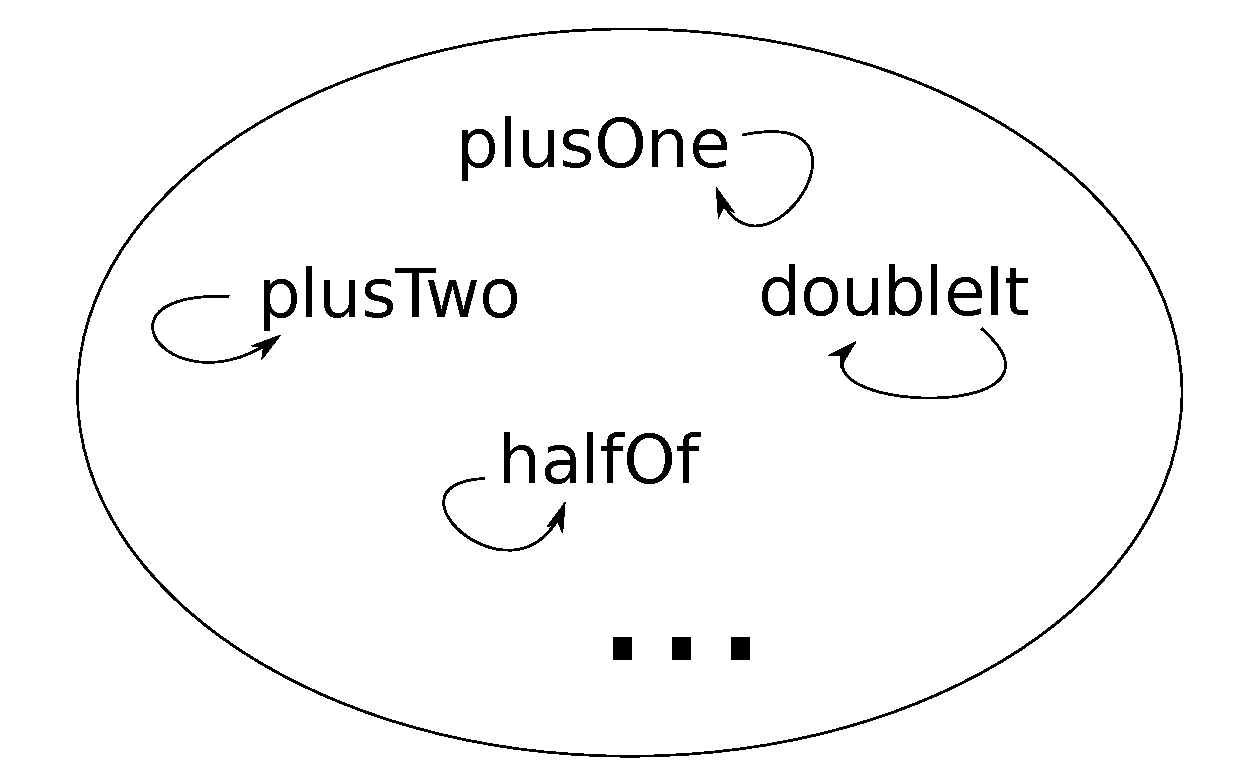
\includegraphics[width=250px]{relation-onetofive-functions}
\end{center}
\end{frame}

% - - - - - - - - - - - - - - - - - - - - - - - - - - - - - - - - - - - - - - - - - - - - - - - - - - - - - - - - - - - - 

\begin{frame}[fragile]
\frametitle{Relationale Aktionen: Typabstraktion}

Ausdrücke sind verwandt, wenn sie bezüglich aller Typrelationen auf alle Typen instanziiert verwandt sind.

\pause
\vspace{36px}

Beispiel:

\begin{minted}{haskell}
t :: forall a. a -> a
\end{minted}

\pause

$\Rightarrow \forall \mathcal{R}.~ \mathcal{R} \rightarrow \mathcal{R}$
\end{frame}

% - - - - - - - - - - - - - - - - - - - - - - - - - - - - - - - - - - - - - - - - - - - - - - - - - - - - - - - - - - - - 

\begin{frame}
\frametitle{Parametrizität}

\begin{Theorem}[Parametrizität]
Ist e ein Ausdruck vom Typ t (also e :: t) und ist $\mathcal{R}$ die zu t konstruierte Typrelation, so gilt
$(e, e) \in \mathcal{R}$.
\end{Theorem}

\end{frame}

% - - - - - - - - - - - - - - - - - - - - - - - - - - - - - - - - - - - - - - - - - - - - - - - - - - - - - - - - - - - - 

\begin{frame}
\frametitle{Parametrizität}

\begin{itemize}
\item Durch Parametrizität lässt sich Aussage für jede Signatur treffen
\item Durch Abrollen der Aussage erhält man freies Theorem
\end{itemize}

\end{frame}

% - - - - - - - - - - - - - - - - - - - - - - - - - - - - - - - - - - - - - - - - - - - - - - - - - - - - - - - - - - - - 


% % % % % % % % % % % % % % % % % % % % % % % % % % % % % % %
\section{Die Bibliothek free-theorems}
% % % % % % % % % % % % % % % % % % % % % % % % % % % % % % %

\begin{frame}
\frametitle{Überblick}
\begin{center}
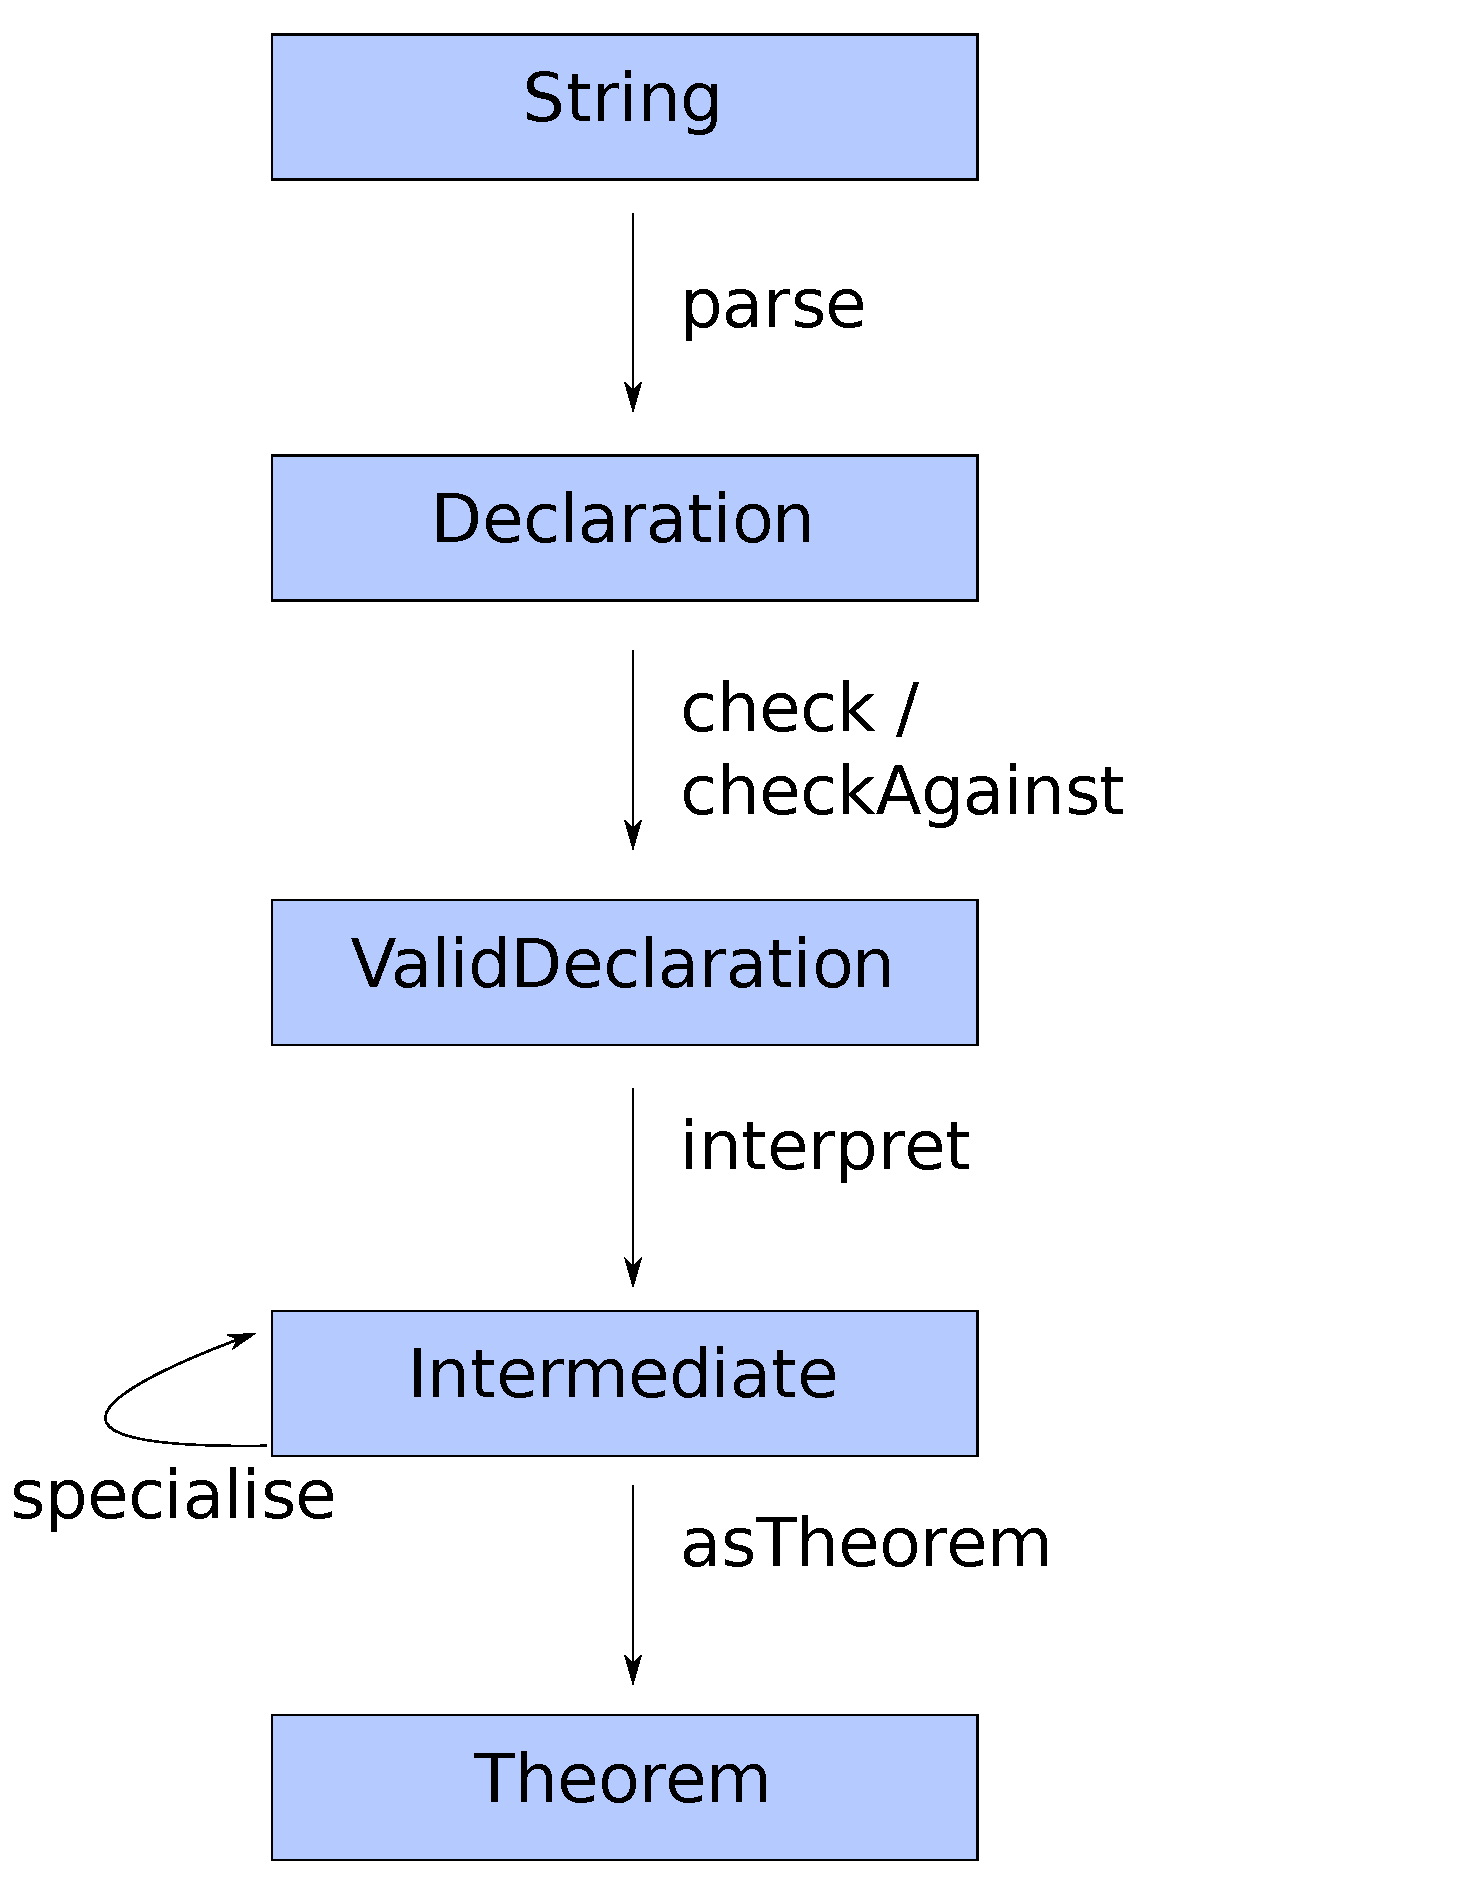
\includegraphics[height=200px]{overview-free-theorems}
\end{center}
\end{frame}

% - - - - - - - - - - - - - - - - - - - - - - - - - - - - - - - - - - - - - - - - - - - - - - - - - - - - - - - - - - - - 

\begin{frame}
\frametitle{Parser}
\begin{center}
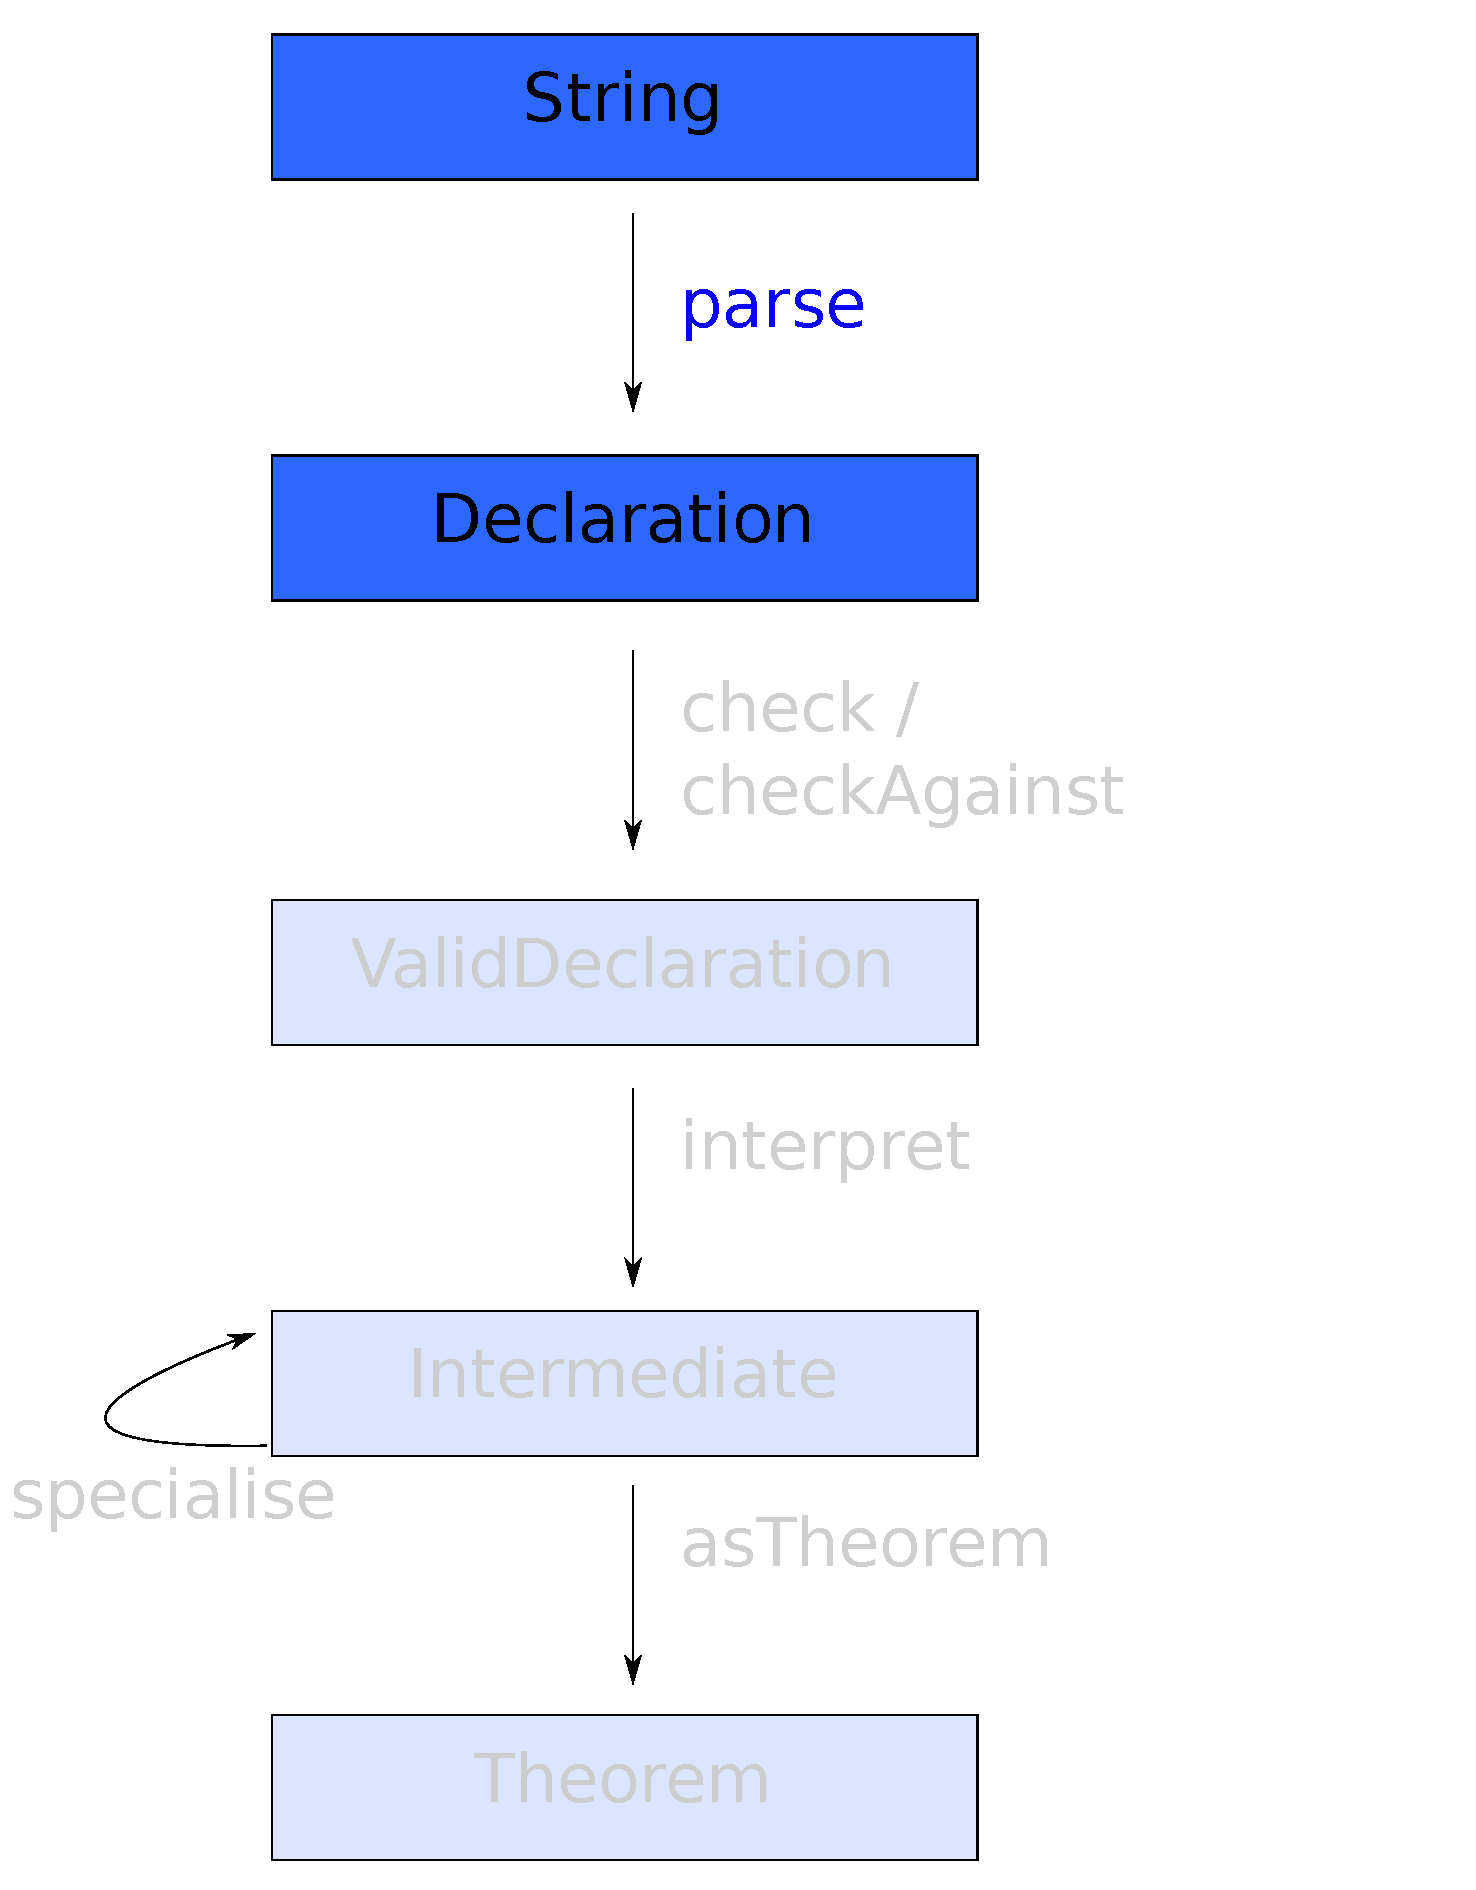
\includegraphics[height=200px]{overview-free-theorems-parse}
\end{center}
\end{frame}

% - - - - - - - - - - - - - - - - - - - - - - - - - - - - - - - - - - - - - - - - - - - - - - - - - - - - - - - - - - - - 

\begin{frame}[fragile]
\frametitle{Parser}
\begin{minted}{haskell}
f :: Functor f => (a -> b) -> f a -> f b
\end{minted}

\pause

\begin{center}
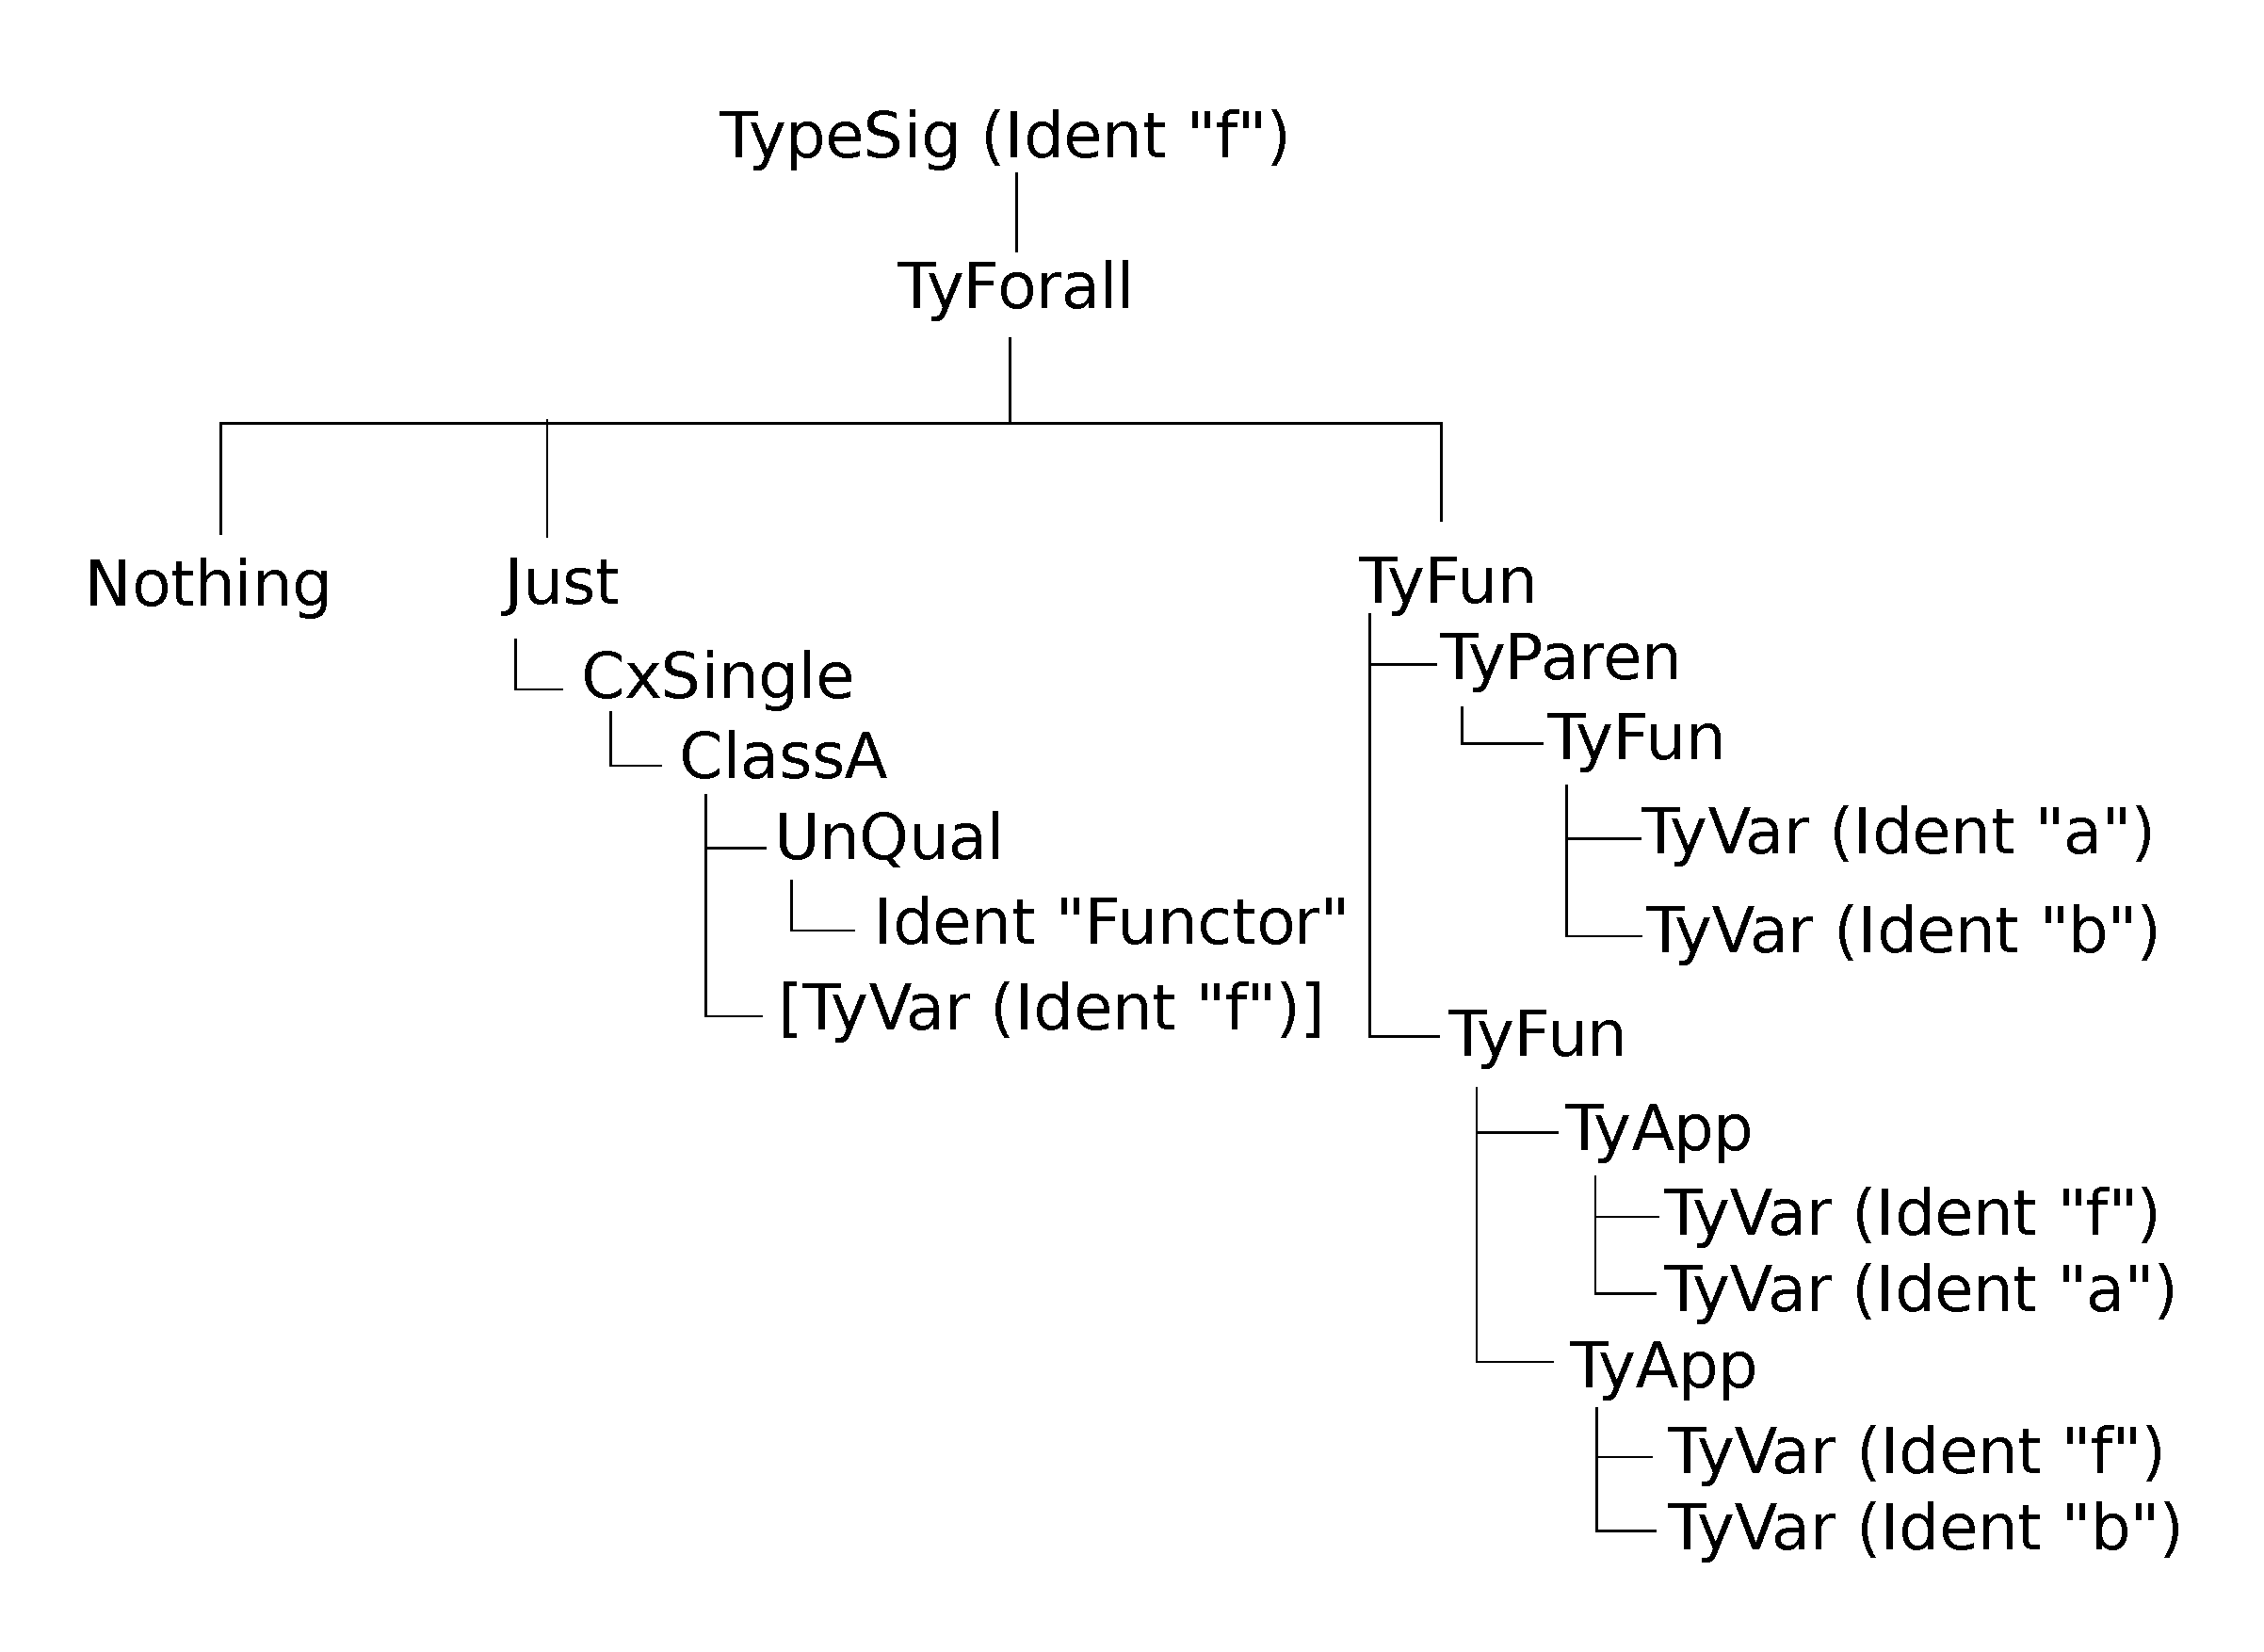
\includegraphics[height=200px]{ast-orig}
\end{center}
\end{frame}

% - - - - - - - - - - - - - - - - - - - - - - - - - - - - - - - - - - - - - - - - - - - - - - - - - - - - - - - - - - - - 

\begin{frame}[fragile]
\frametitle{BasicSyntax}
\begin{minted}{haskell}
f :: Functor f => (a -> b) -> f a -> f b
\end{minted}

\begin{center}
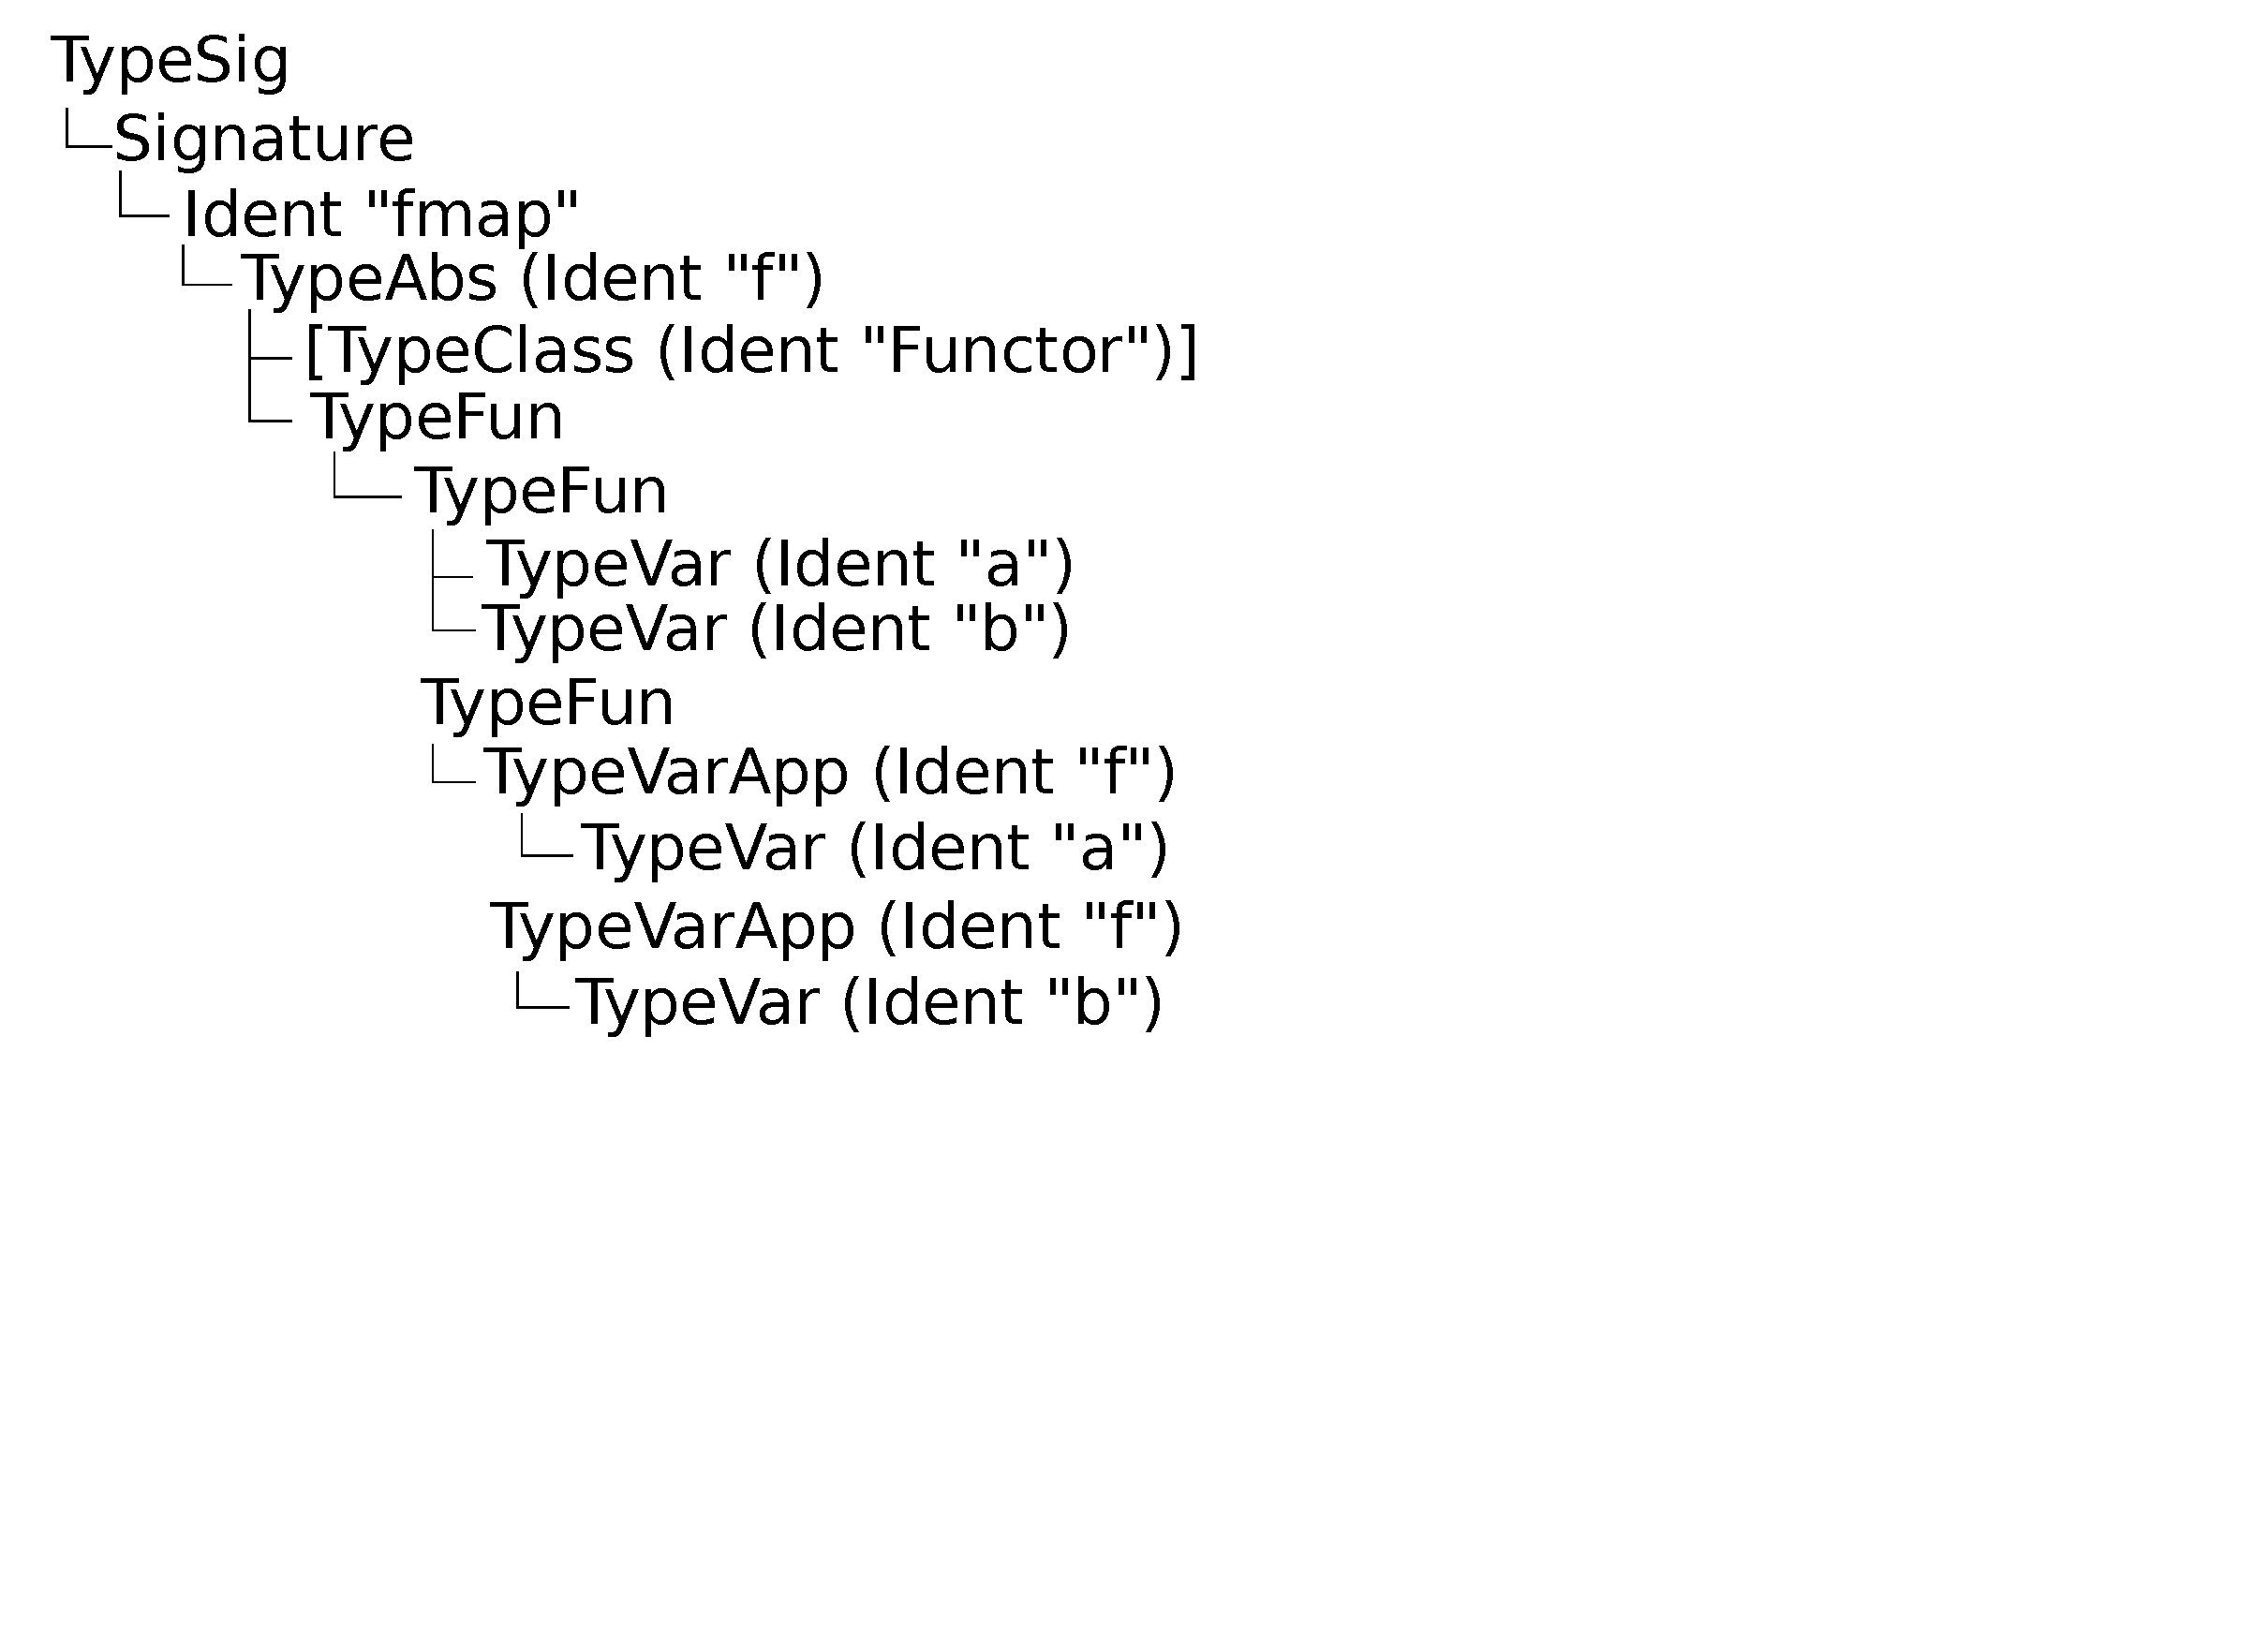
\includegraphics[height=200px]{ast-simple}
\end{center}
\end{frame}

% - - - - - - - - - - - - - - - - - - - - - - - - - - - - - - - - - - - - - - - - - - - - - - - - - - - - - - - - - - - - 

\begin{frame}
\frametitle{Checks}
\begin{center}
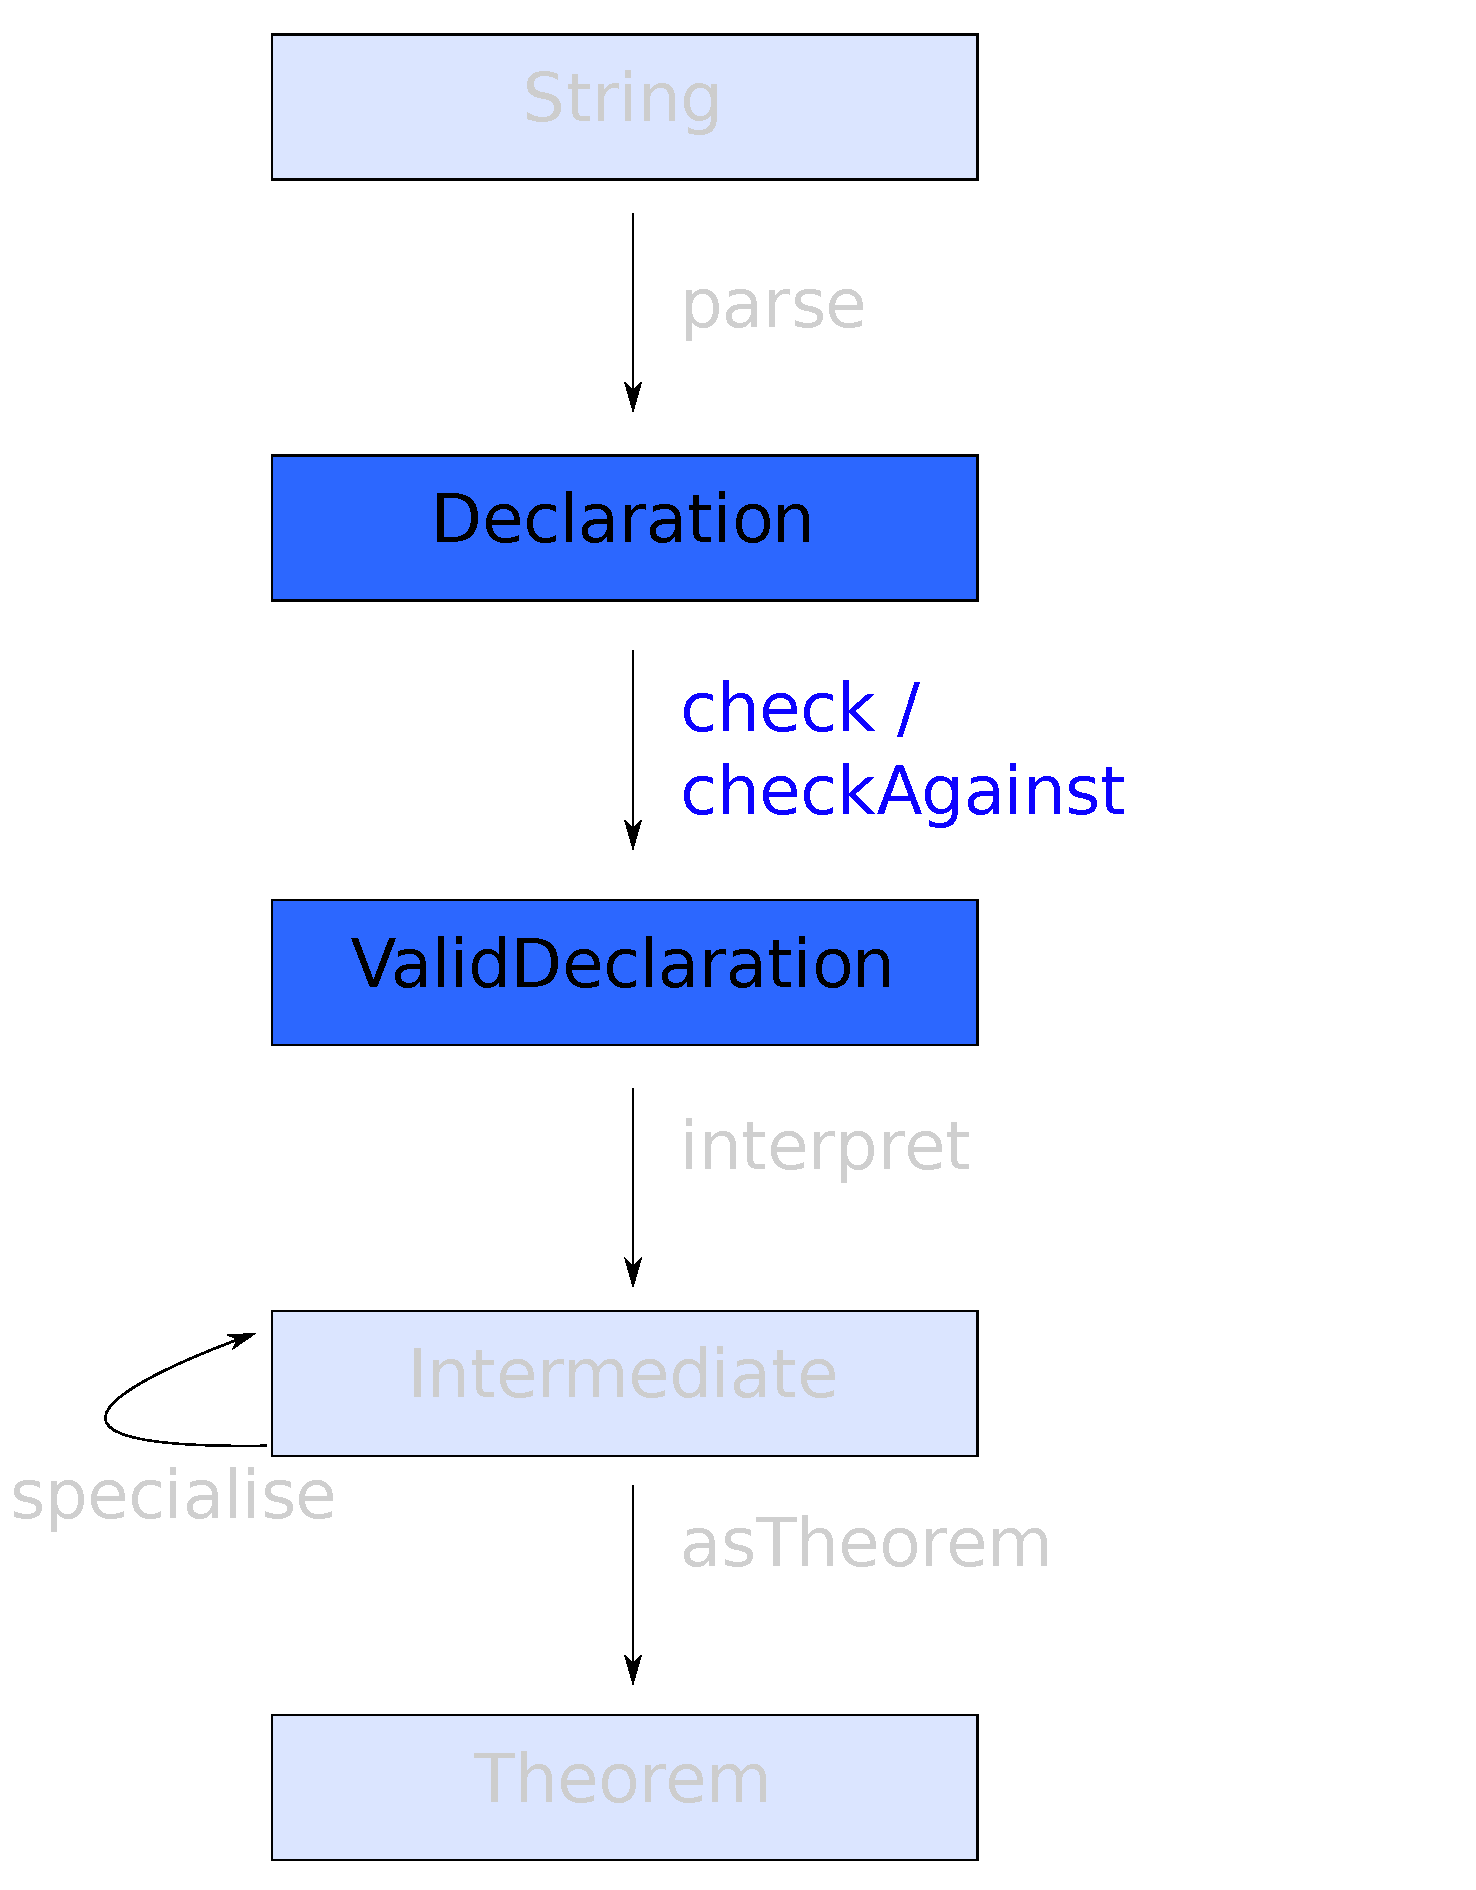
\includegraphics[height=200px]{overview-free-theorems-check}
\end{center}
\end{frame}

% - - - - - - - - - - - - - - - - - - - - - - - - - - - - - - - - - - - - - - - - - - - - - - - - - - - - - - - - - - - - 

\begin{frame}[fragile]
\frametitle{BasicSyntax nach Check}
\begin{minted}{haskell}
f :: Functor f => (a -> b) -> f a -> f b
\end{minted}

\begin{center}
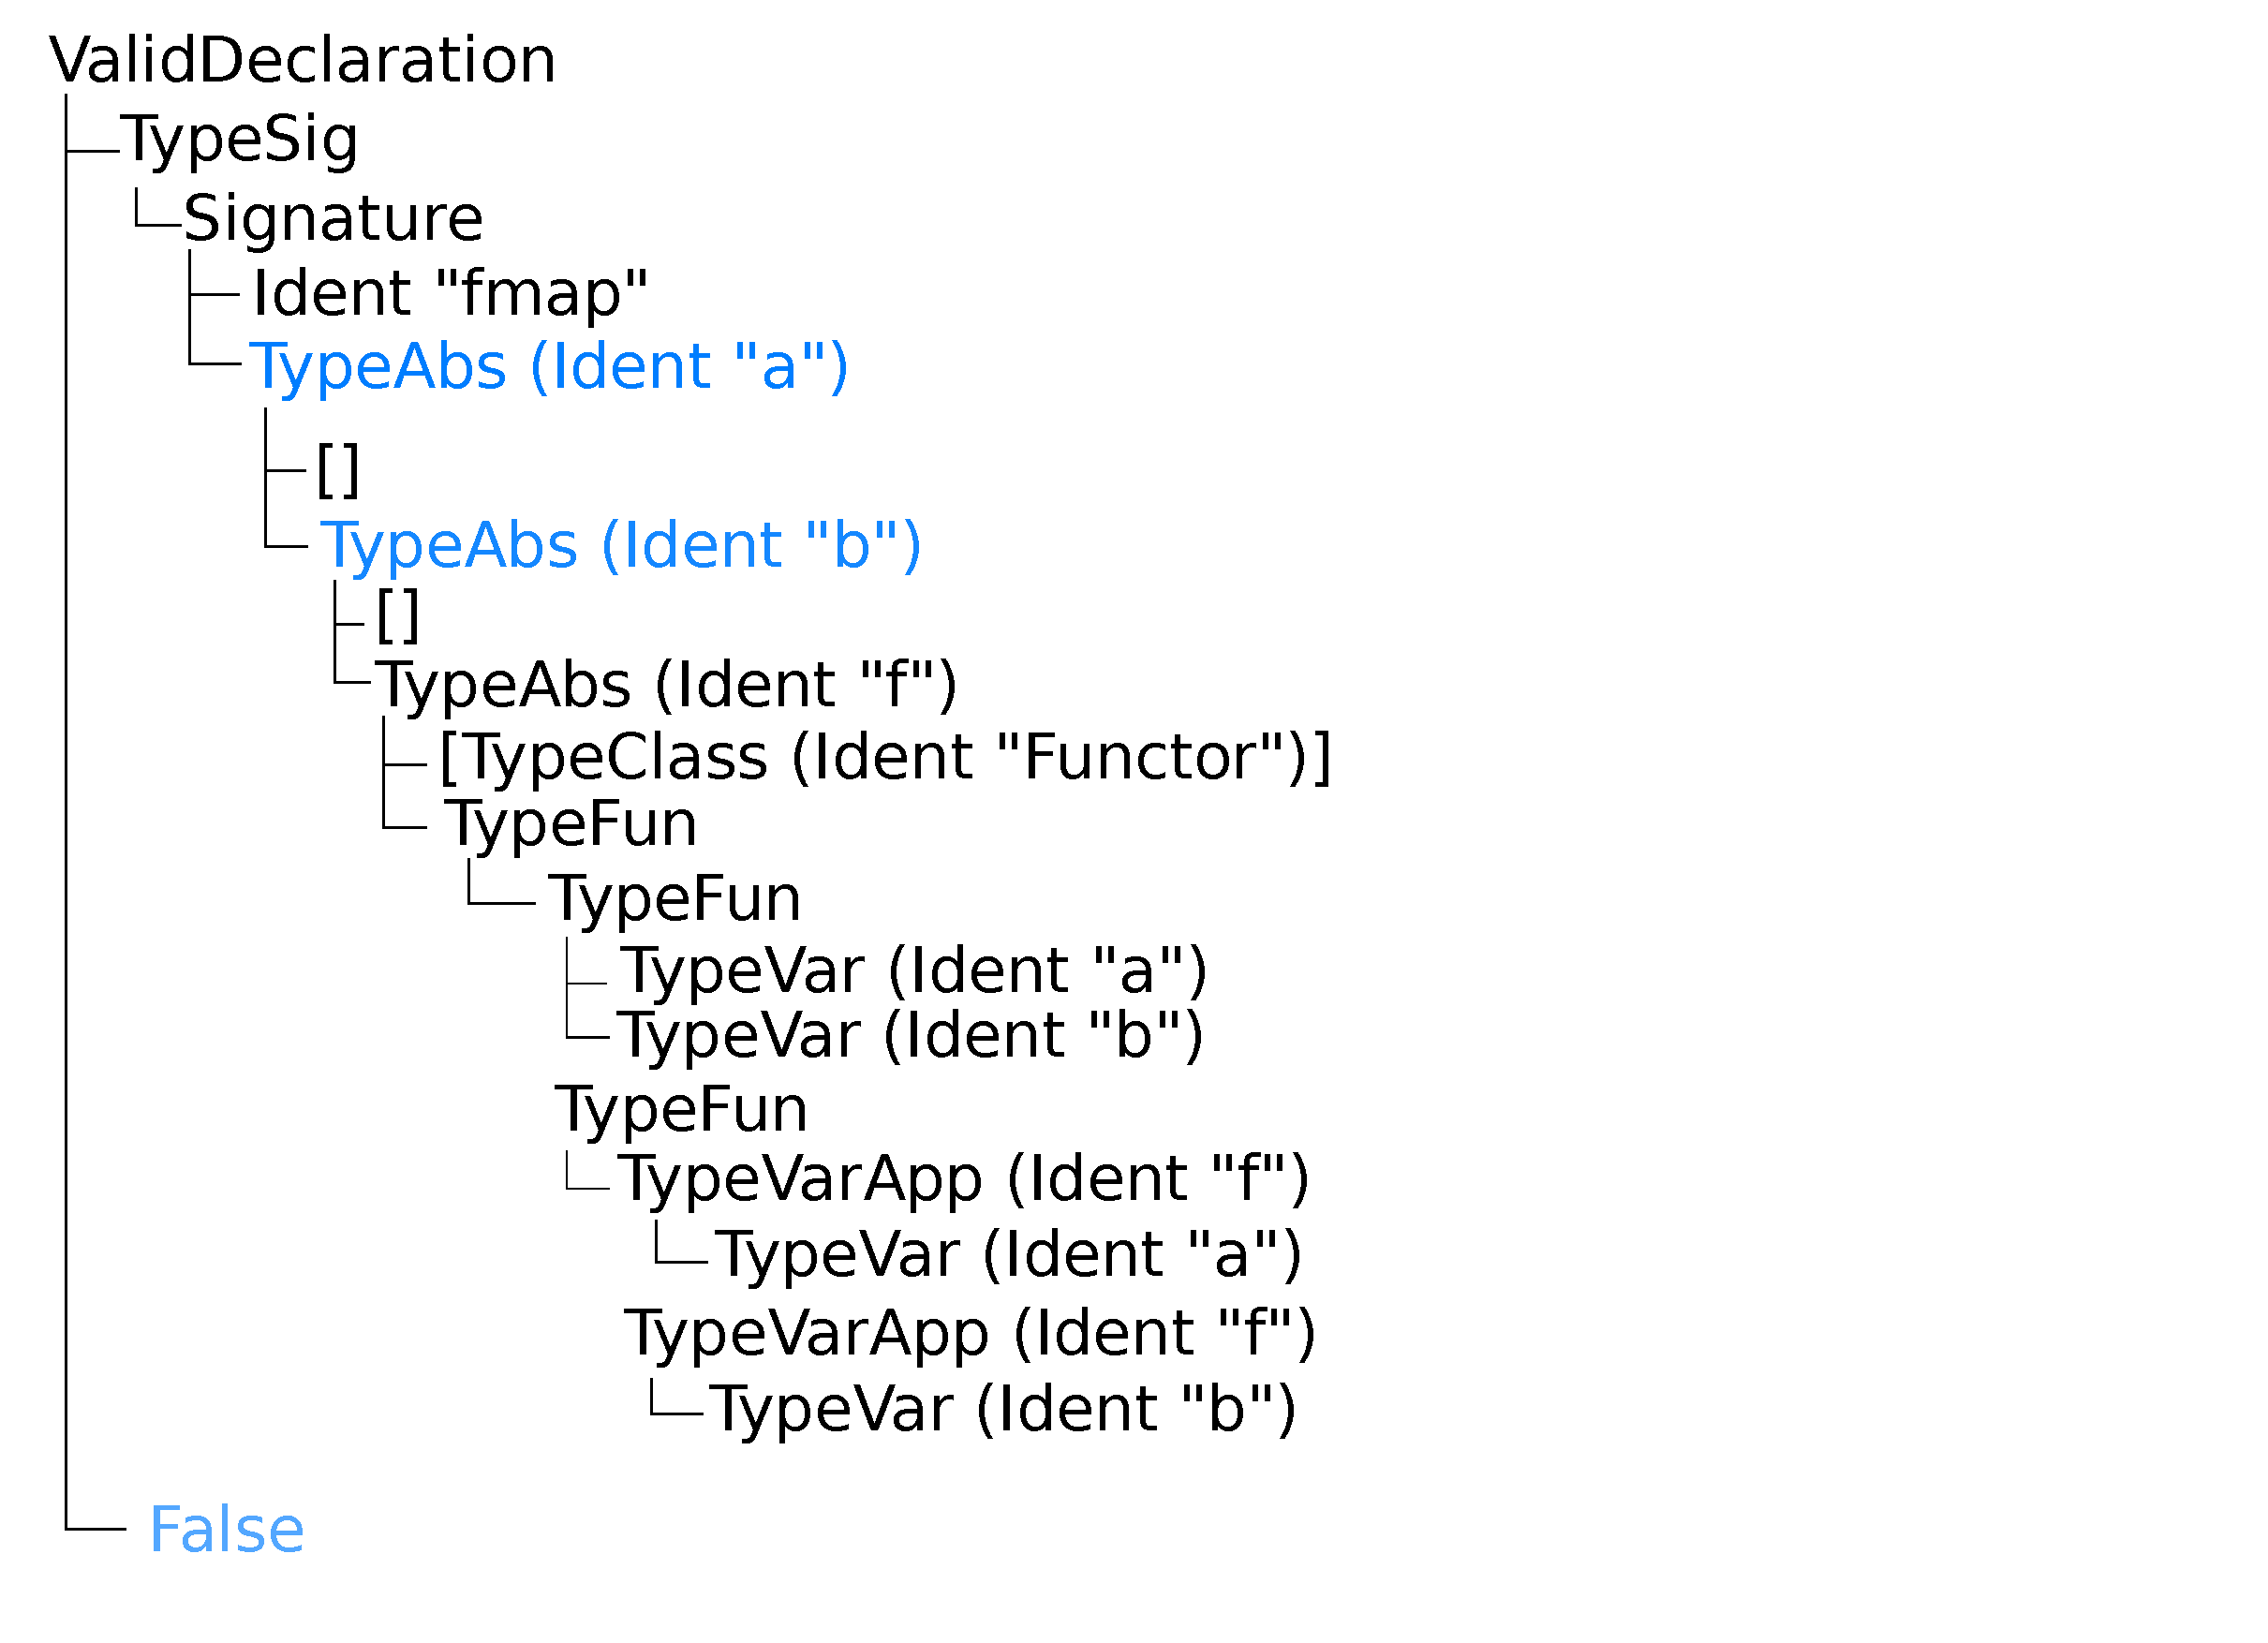
\includegraphics[height=200px]{ast-simple-checked}
\end{center}
\end{frame}

% - - - - - - - - - - - - - - - - - - - - - - - - - - - - - - - - - - - - - - - - - - - - - - - - - - - - - - - - - - - - 

\begin{frame}
\frametitle{Checks: Beispiele}

Beispiele für Überprüfungen

\begin{itemize}
\item Variablen der rechten Seite kommen auf der linken Seite vor
\item Keine doppelten Funktionsvariablen
\item Keine doppelten Funktionsdeklarationen
\end{itemize}

\end{frame}

% - - - - - - - - - - - - - - - - - - - - - - - - - - - - - - - - - - - - - - - - - - - - - - - - - - - - - - - - - - - - 

\begin{frame}[fragile]
\frametitle{Checks: Beispiele}

Typvariable wird auf die korrekte Anzahl an Typparametern angewandt

\begin{minted}{haskell}
f :: Functor f => Int -> f -- FEHLER
\end{minted}

\end{frame}

% - - - - - - - - - - - - - - - - - - - - - - - - - - - - - - - - - - - - - - - - - - - - - - - - - - - - - - - - - - - - 

\begin{frame}[fragile]
\frametitle{Checks: Beispiele}

Typvariable einer Typkonstruktorklasse wird immer auf gleiche Parameterzahl angewandt

\begin{minted}{haskell}
class SomeClass c where
   fun1 :: c a -> c a
   fun2 :: c -> Int -- FEHLER
\end{minted}

\end{frame}

% - - - - - - - - - - - - - - - - - - - - - - - - - - - - - - - - - - - - - - - - - - - - - - - - - - - - - - - - - - - - 

\begin{frame}
\frametitle{Interpretation als Relation}
\begin{center}
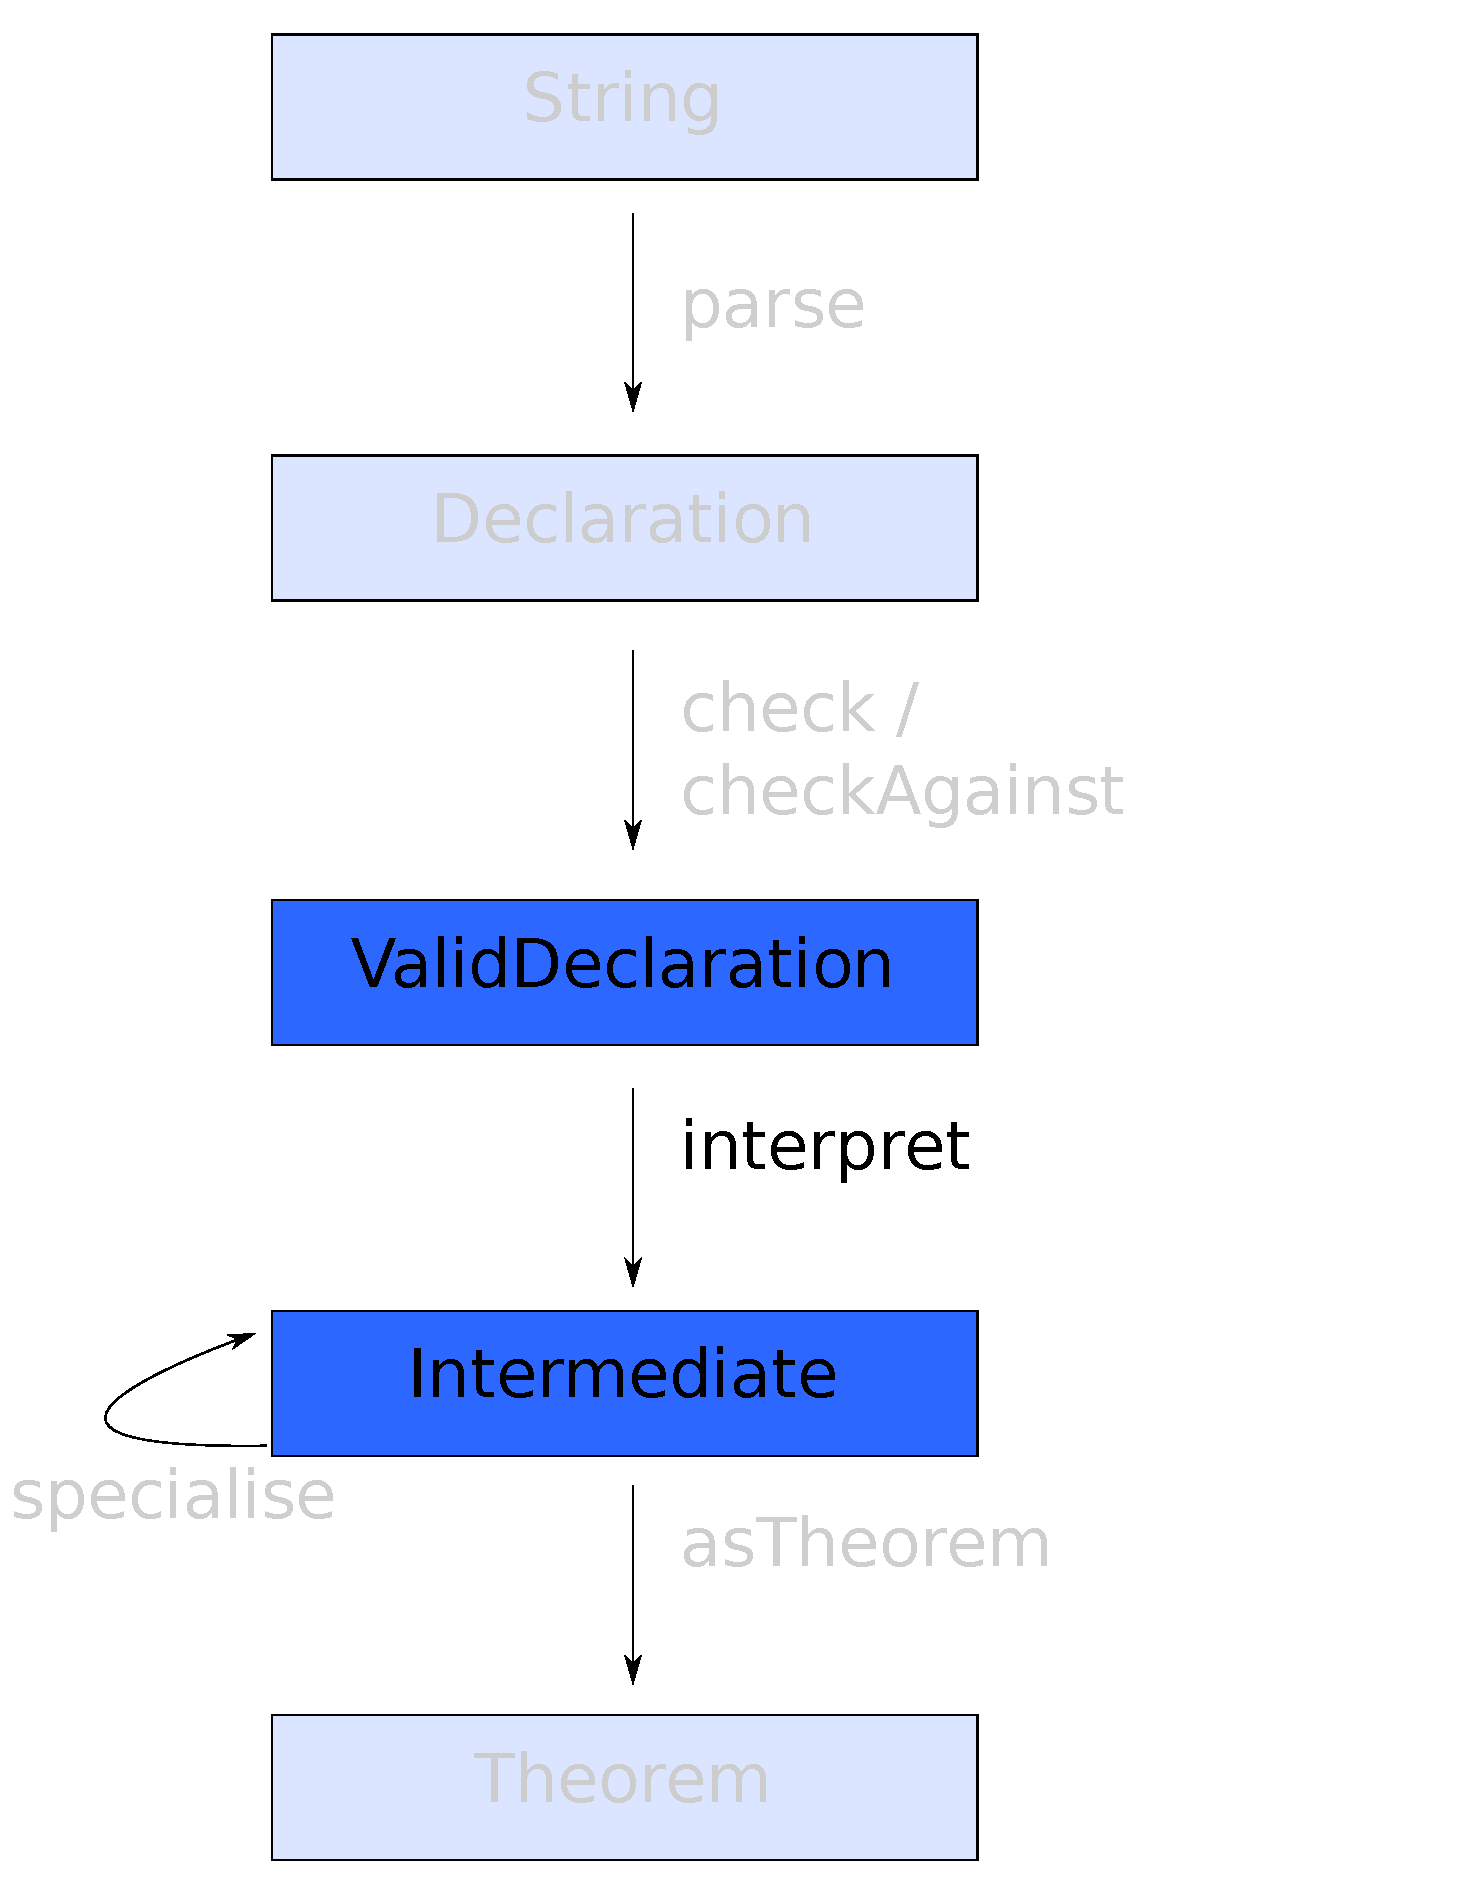
\includegraphics[height=200px]{overview-free-theorems-interpret}
\end{center}
\end{frame}

% - - - - - - - - - - - - - - - - - - - - - - - - - - - - - - - - - - - - - - - - - - - - - - - - - - - - - - - - - - - - 

\begin{frame}
\frametitle{Interpretation als Relation}

\begin{center}
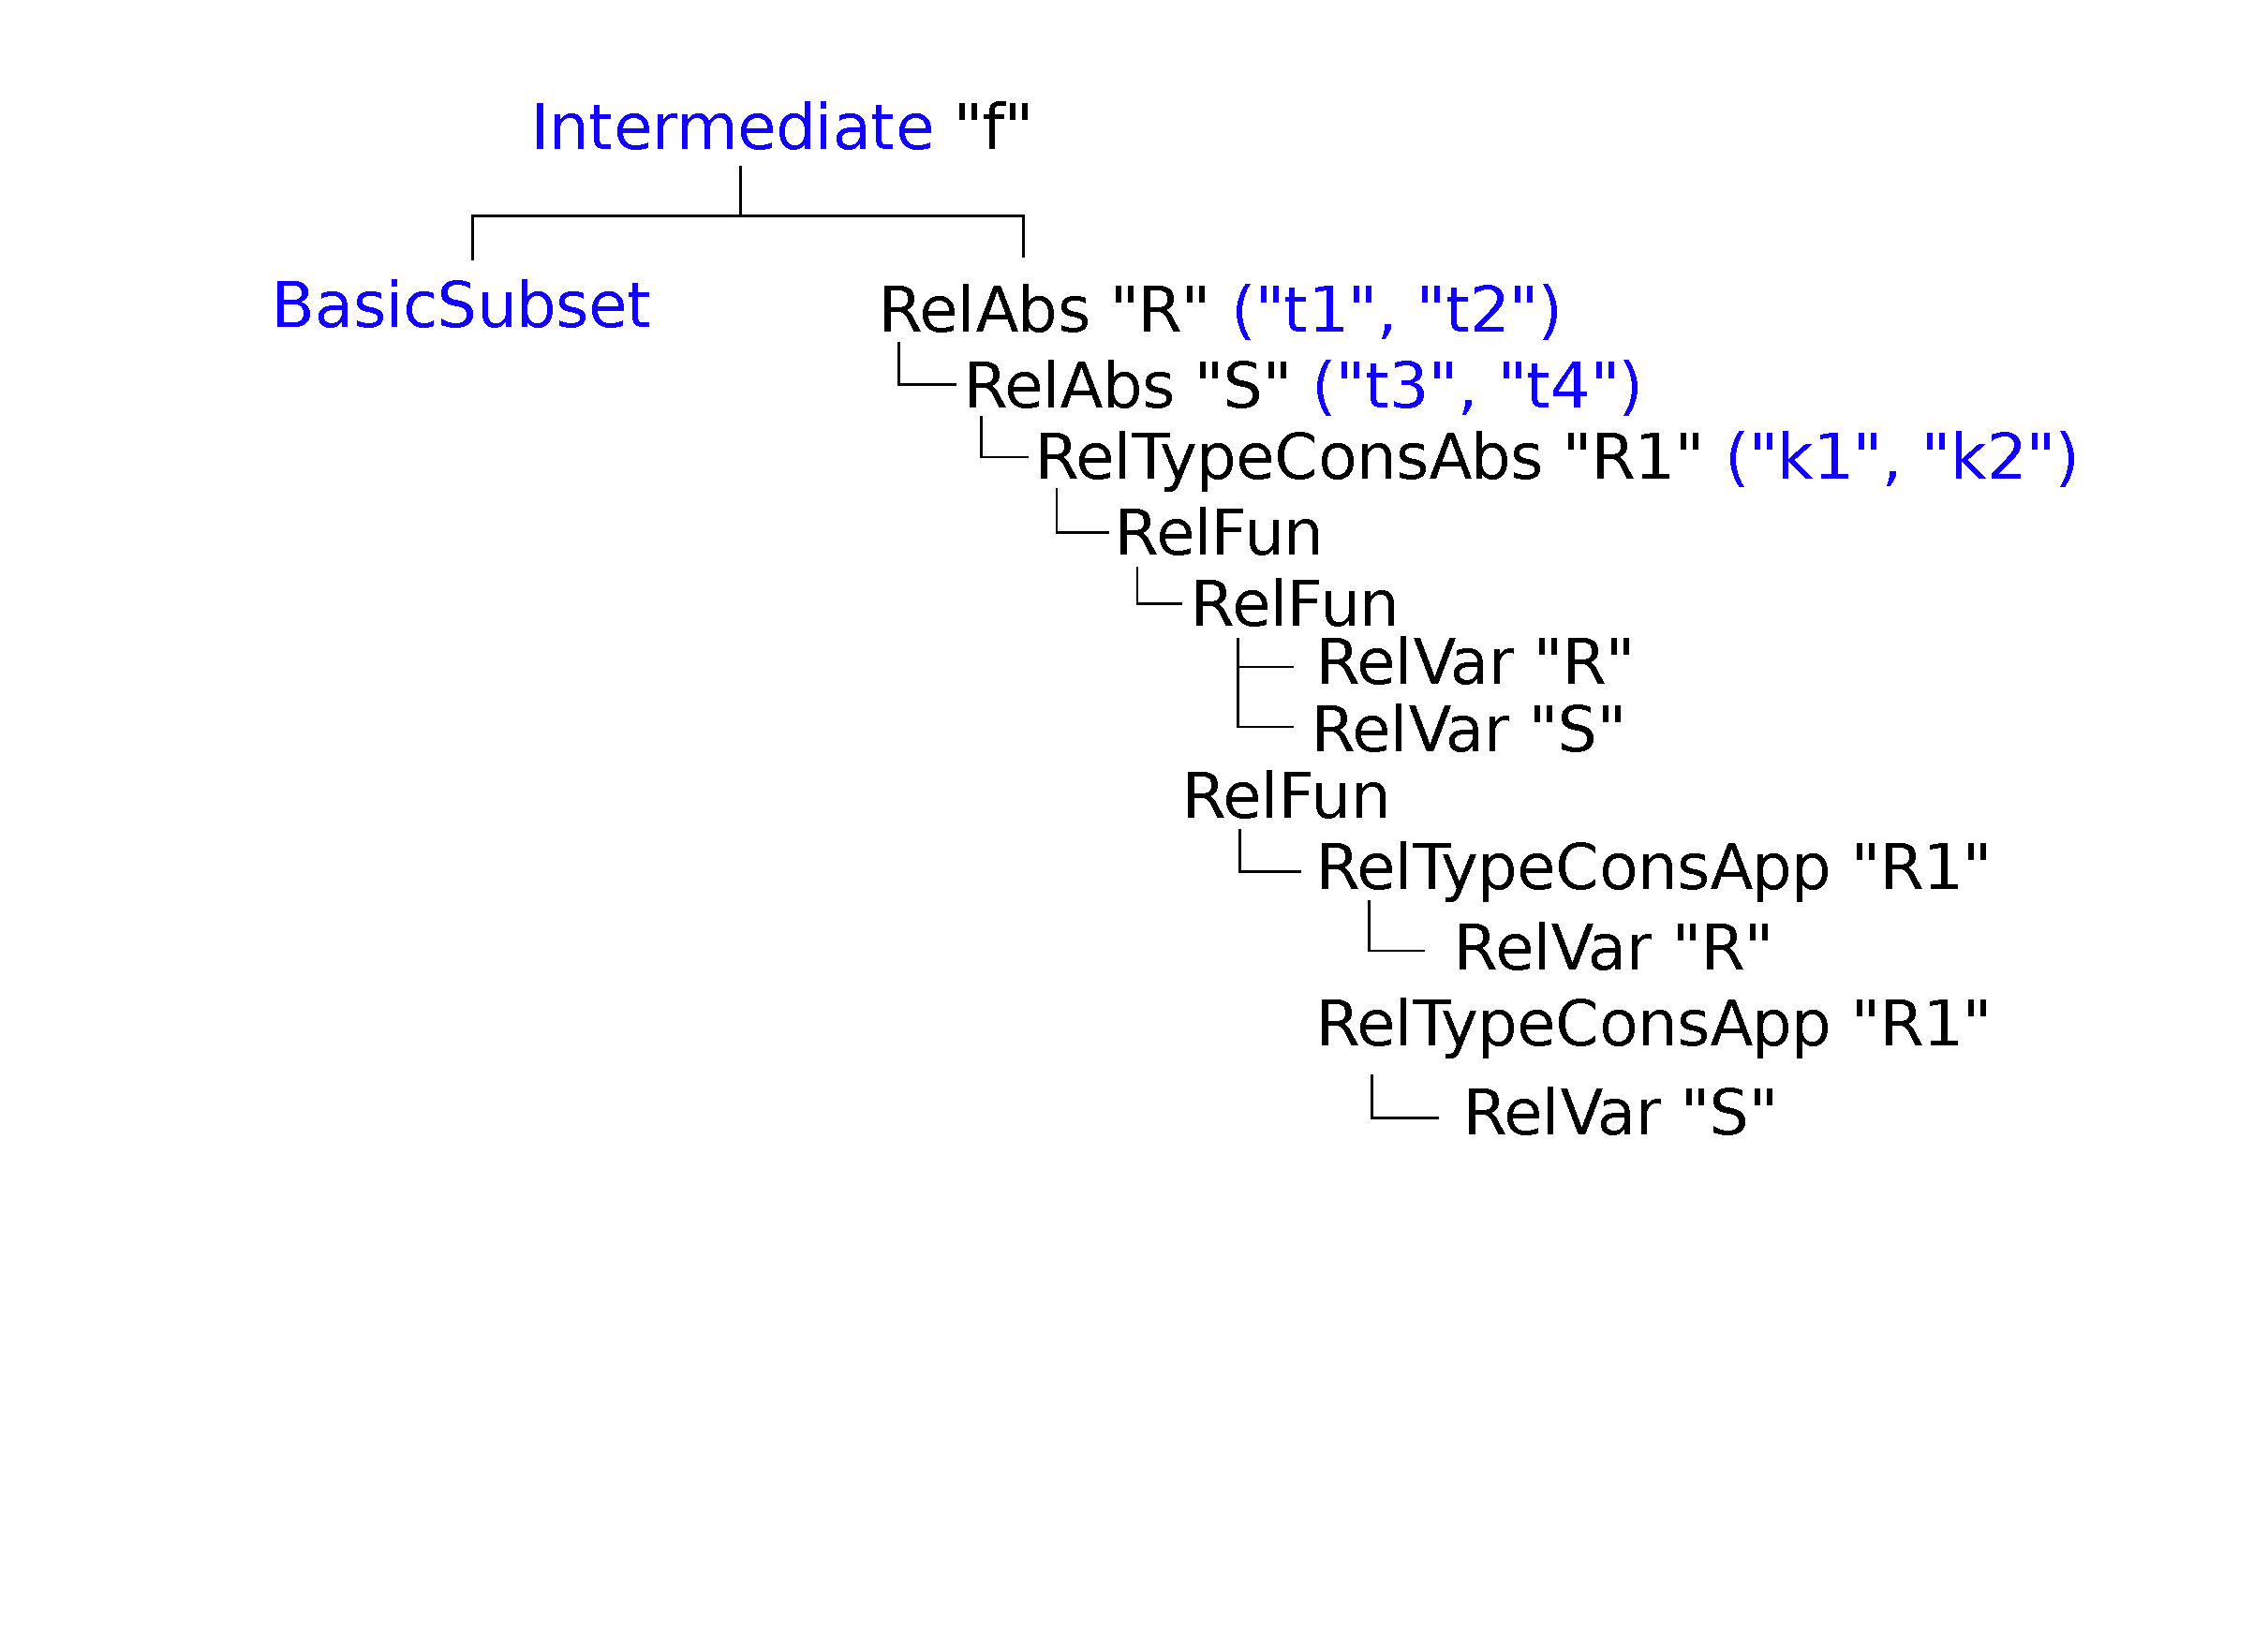
\includegraphics[width=250px]{intermediate}
\end{center}

\end{frame}

% - - - - - - - - - - - - - - - - - - - - - - - - - - - - - - - - - - - - - - - - - - - - - - - - - - - - - - - - - - - - 

\begin{frame}
\frametitle{Generierung des freien Theorems durch Abrollen}
\begin{center}
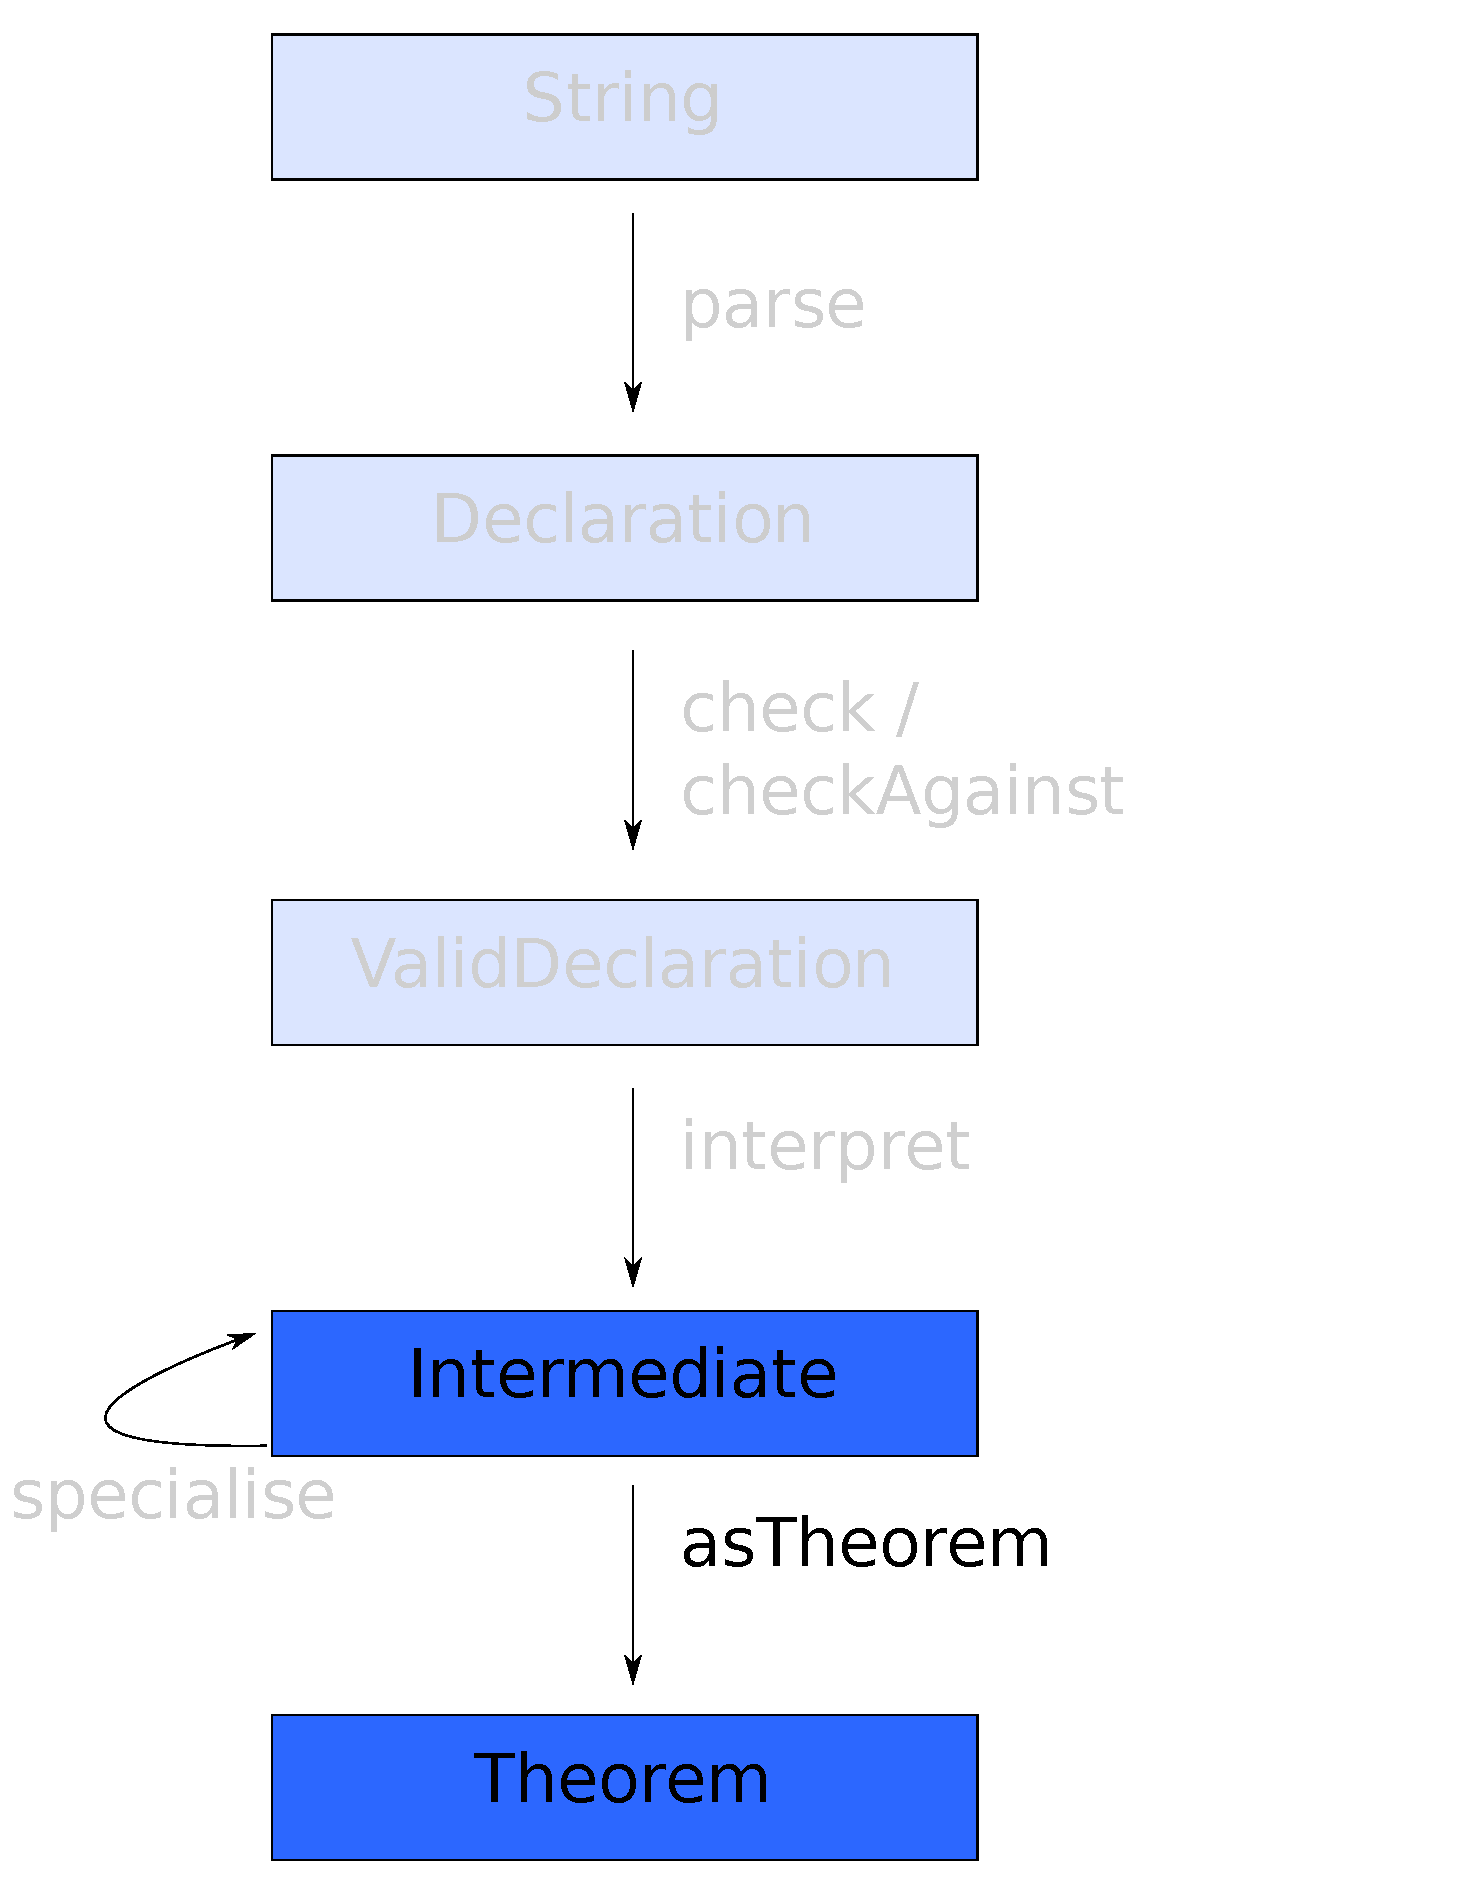
\includegraphics[height=200px]{overview-free-theorems-astheorem}
\end{center}
\end{frame}

% - - - - - - - - - - - - - - - - - - - - - - - - - - - - - - - - - - - - - - - - - - - - - - - - - - - - - - - - - - - - 

\begin{frame}[fragile]
\frametitle{Generierung des freien Theorems durch Abrollen}

\begin{minted}{text}
forall t1,t2 in TYPES, R in REL(t1,t2).
 forall t3,t4 in TYPES, S in REL(t3,t4).
  forall k1,k2 in (* -> *), R1 : k1 <=> k2,
           R1 respects Functor.
   forall p :: t1 -> t3.
    forall q :: t2 -> t4.
     (forall (x, y) in R. (p x, q y) in S)
     ==> (forall (z, v) in R1 R.
           (f_{t1}_{t3}_{k1} p z,
            f_{t2}_{t4}_{k2} q v) in R1 S)
\end{minted}
\end{frame}

% - - - - - - - - - - - - - - - - - - - - - - - - - - - - - - - - - - - - - - - - - - - - - - - - - - - - - - - - - - - - 

%\begin{frame}
%\frametitle{Überblick}
%\begin{columns}
%\begin{column}{0.4\textwidth}
%    \begin{center}
%	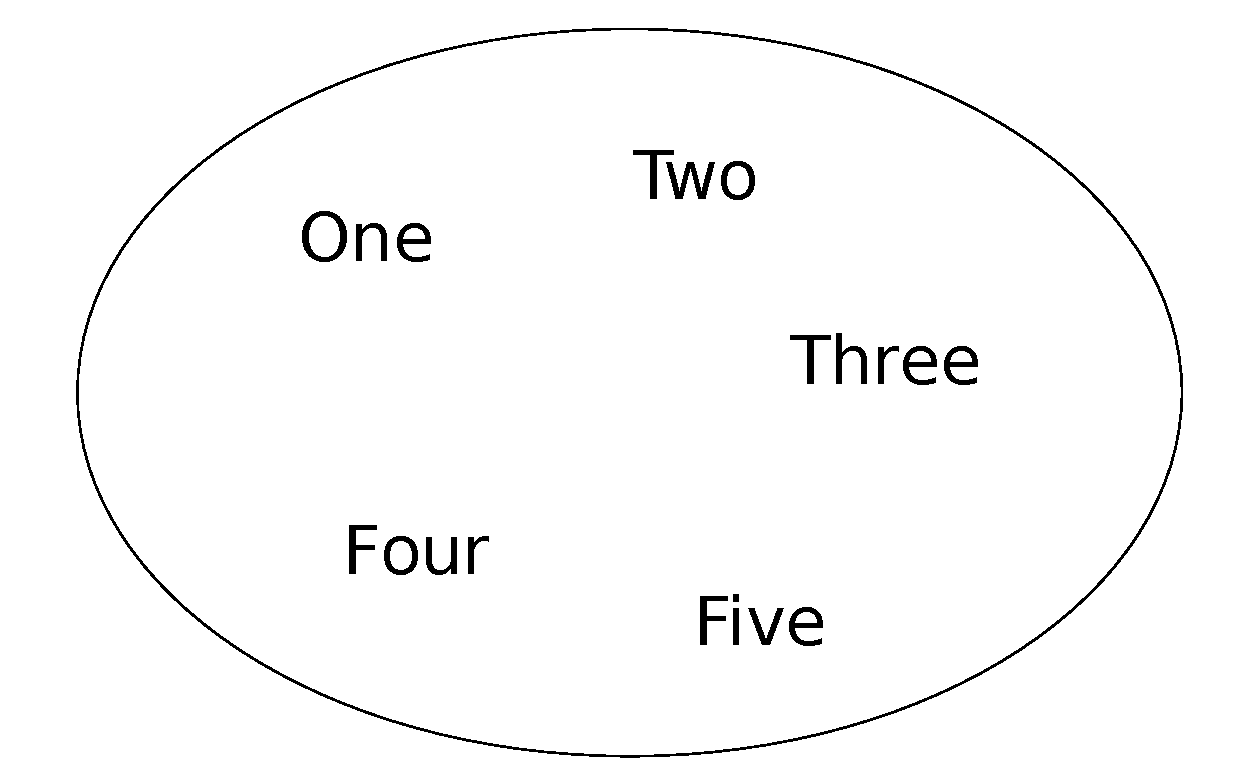
\includegraphics[height=200px]{menge-onetofive}
%     \end{center}
%\end{column}
%\begin{column}{0.6\textwidth}
%\end{column}
%\end{columns}
%\end{frame}

% - - - - - - - - - - - - - - - - - - - - - - - - - - - - - - - - - - - - - - - - - - - - - - - - - - - - - - - - - - - - 

% % % % % % % % % % % % % % % % % % % % % % % % % % % % % % %
\section{free-theorems in Aktion}
% % % % % % % % % % % % % % % % % % % % % % % % % % % % % % %
  
%  \begin{frame}
%  \frametitle{free-theorems in Aktion}
%  \end{frame}
  
\begin{frame}
\vfill
\centering
\begin{beamercolorbox}[sep=8pt,center,shadow=true,rounded=true]{title}
\usebeamerfont{title}Vielen Dank für die Aufmerksamkeit\par%
\end{beamercolorbox}
\vfill
\end{frame}

\end{document}